\chapter{รายละเอียดการปฏิบัติงาน}
\thispagestyle{empty}
\label{chapter:coop-detail}

\section{ตำแหน่งงาน}
    Junior Mobile Developer

\section{หน้าที่ของงานที่ได้รับมอบหมาย}
    \begin{enumerate}
        \item ออกแบบ Sequence Diagram ของกระบวนการจองซื้อหุ้นกู้ในส่วนต่าง ๆ
        \item พัฒนา Website Operation Tools สำหรับการจัดการหุ้นกู้
        \item พัฒนา แอปพลิเคชัน ซีไอเอ็มบีไทยดิจิตอลแบงก์กิ้ง ในส่วนการจองซื้อหุ้นกู้บนระบบปฏิบัติการ Android
        \item พัฒนา แอปพลิเคชัน ซีไอเอ็มบีไทยดิจิตอลแบงก์กิ้ง ในส่วนการจองซื้อหุ้นกู้บนระบบปฏิบัติการ iOS
    \end{enumerate}

\section{ขอบเขตของงานที่ได้รับมอบหมาย}
    นักศึกษาได้มีส่วนร่วมช่วยพัฒนาโมบายล์แอพพลิ
    เคชั่นบนระบบปฏิบัติการ Android และ iOS ในหน้าต่าง ๆ 
    และเว็บไซต์ Operation Tools ได้แก่
    \subsection{โมบายล์แอปพลิเคชัน}
        \begin{enumerate}
            \item หน้า Bond home
            \item หน้า Term and Condition
            \item หน้า Bond transaction history
            \item หน้า Bond detail
            \item หน้า CSA Questionnaire
            \item หน้า Factsheet
            \item หน้า Warning List (Risk Acceptance)
            \item หน้า Payment Confirmation
            \item หน้า Benificial Information
            \item หน้า Receive Bond Information
            \item หน้า Review Bond Booking detail
            \item หน้า Passcode
            \item หน้า Receipt
        \end{enumerate}

    \subsection{เว็บไซต์}
        \begin{enumerate}
            \item หน้า Bond Management
            \item หน้า Add Bond
            \item หน้า Edit Bond
        \end{enumerate}

\section{ทฤษฎีที่เกี่ยวข้อง}
    \subsection{หุ้นกู้}
        หุ้นกู้ คือตั๋วสัญญาใช้เงินระยะยาวประเภทหนึ่งที่ออกโดยผู้กู้ ซึ่งระบุว่าผู้กู้ ได้กู้ยืมเงินจำนวนหนึ่งจากผู้ซื้อ หรือผู้ถือหุ้นกู้ โดยผู้กู้สัญญาว่าจะจ่ายคืนเงินจำนวนดังกล่าวในอนาคตและจ่ายดอกเบี้ยเป็นรายงวดตามวันที่กำหนดไว้ตลอดอายุหุ้นกู้ ผู้ถือหุ้นกู้จะมีสภาพเป็นเจ้าหนี้ของบริษัทที่ออกหุ้นกู้นั้น
        หุ้นกู้ที่ออกจำหน่ายจะต้องระบุข้อมูล ดังนี้
        \begin{itemize}
            \item[-] ระยะเวลาครบกำหนดไถ่ถอน หรืออายุหุ้นกู้
            \item[-] มูลค่าที่ตราไว้ หรือ มูลค่าเมื่อครบกำหนดไถ่ถอน ซึ่งเป็นเงินต้นที่ผู้กู้ต้องชำระคืน ณ วันครบกำหนดไถ่ถอน โดยปกติจะเท่ากับ 1,000 บาท
            \item[-] อัตราดอกเบี้ยที่ระบุไว้บนใบหุ้นกู้ ซึ่งแสดงถึงร้อยละของมูลค่าที่ตราไว้ โดยมักจะจ่ายเป็นรายปีหรือรายครึ่งปี
        \end{itemize}
        หุ้นกู้จัดเป็นหลักทรัพย์ที่ให้รายได้ประจำ เนื่องจากการจ่ายดอกเบี้ยและชำระคืนเงินต้นของหุ้นกู้ ได้ระบุไว้แน่นอน ณ เวลาที่ออกและกำหนดเป็นจำนวนเงินคงที่ ตลอดอายุหุ้นกู้ ดังนั้นผู้ซื้อหรือผู้ถือหุ้นกู้จะทราบถึงกระแสเงินสดในอนาคตที่จะได้รับนับ จากวันที่ซื้อจนถึงวันครบกำหนดไถ่ถอน\cite{bond}

    \subsection{Microservice}
        Microservice คือสถาปัตยกรรมที่ใช้ในการพัฒนาซอฟต์แวร์โดยมีการทำงานที่จะแยกให้แต่ละ Service ไม่ขึ้นต่อกัน (Loosely coupled) และรวบรวมการทำงานของ Service ให้การทำงานที่เกี่ยวข้องอยู่ร่วมกันโดยพยายามไม่ให้แยกออกจากกันมากที่สุด
        เพื่อหลีกเลี่ยงผลกระทบจากแก้ไข (High Cohesion) โดยแต่ละ Service จะถูกแบ่งตามความต้องการของลูกค้า หรือแบ่งตามภาคธุรกิจ
        โดยลักษณะการทำงานของ Microservice ที่ดีมีดังนี้
        \begin{itemize}
            \item[-] มีขอบเขตของปัญหาที่เล็ก
            \item[-] สามารถ Build และ Deploy ได้ด้วยตัวเองไม่ขึ้นกับ Service อื่น
            \item[-] สามารถทำงานบน Process ของตัวเองได้โดยไม่ต้องพึ่ง Process จาก Service อื่น ๆ
            \item[-] สามารถประยุกต์ใช้ได้กับส่วนอื่น ๆ โดยสื่อสารผ่าน Interface ที่กำหนด
            \item[-] มีที่เก็บข้อมูลของตัวเองเพื่อให้เป็นอิสระทางข้อมูลไม่ต้องใช้ทรัพยากรจาก Service อื่น
        \end{itemize}

    \subsection{Agile}
        Agile เป็นแนวคิดในการทำงาน(ไม่ใช่รูปแบบหรือขั้นตอนในการทำงาน)โดยที่จะเน้นการสื่อสารและปฏิสัมพันธ์กันระหว่างเพื่อนร่วมทีมมากกว่านำเครื่องมือต่าง ๆ มาช่วย
        เน้นการทำผลิตภัณฑ์มากกว่าทำเอกสาร เน้นการตอบสนองลูกค้ามากกว่าการทำตามสัญญา และเน้นการปรับปรุงพัฒนามากกว่าการทำตามแผนที่วางเอาไว้
        โดยผลิตภัณฑ์ถูกพัฒนาขึ้นเพื่อแก้ไขปัญหาหรือตอบสนองความต้องการของลูกค้า เราจึงนำมาระบุให้ชัดเจนในรูปแบบของ User Story
        และตำแหน่งที่สำคัญในที่ทีมพัฒนาแบบ Agile มีดังนี้
        \begin{itemize}
            \item[-] Stakeholders แสดงความต้องการ(Requirement)
            \item[-] Product Owner (PO) เก็บ Requirement มาจาก Stakeholders
            \item[-] Developer Lead นำ Requirement มาแปลงเป็น User Story
            \item[-] Developer (Dev) นำ Design ที่ออกแบบไว้มาพัฒนาเป็นผลิตภัณฑ์จริง
            \item[-] Quality Assurance (QA) นำ Acceptance Criteria มาขยาย Happy และ Unhappy Case ให้ครอบคลุมพฤติกรรมการใช้งานทุกรูปแบบที่เป็นไปได้ให้ได้มากที่สุด นำผลิตภัณฑ์มาทดสอบให้เป็นไปตาม BDD / Test Case ที่ออกแบบไว้
            \item[-] Operation (Ops) นำผลิตภัณฑ์ที่ผ่านการทดสอบแล้วไปส่งมอบให้ลูกค้าสามารถเข้ามาใช้งานได้
        \end{itemize}

    \subsection{Scrum}
        \begin{figure}[H]
            \centering
            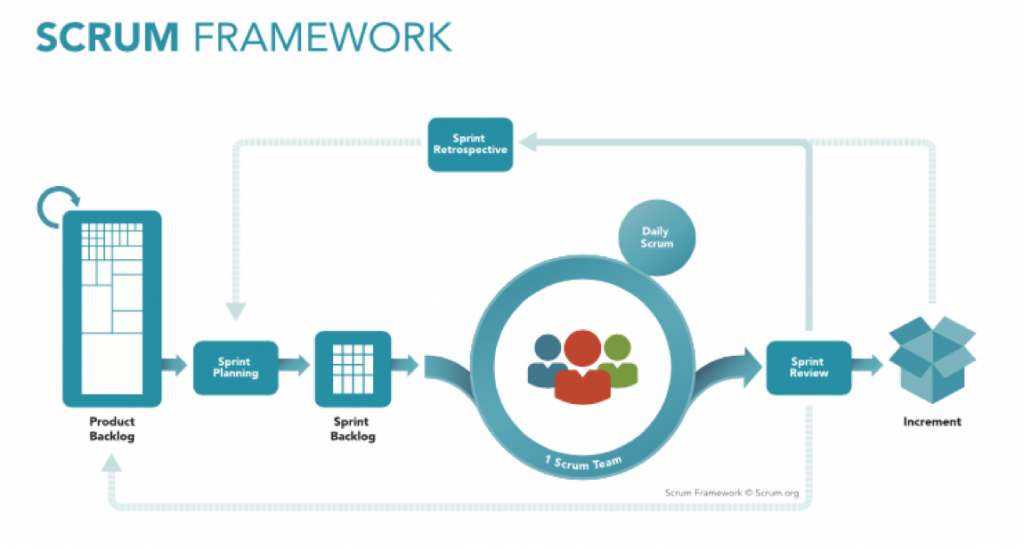
\includegraphics[width=1\textwidth]{scrum-framework}
            \caption{โครงสร้างการทำงานแบบ Scrum}\label{scrum-framework}
        \end{figure}
        Scrum เป็นรูปแบบการพัฒนาซอฟตฺแวร์ที่นำแนวคิดในการทำงานแบบ Agile มาปรับมาปรับใช้โดยเน้นเรื่องการส่งมอบงานให้ลูกค้าแบบเป็นระยะ ๆ 
        เพื่อที่จะได้รับผลตอบรับจากลูกค้าและนำมาปรับแก้ไขให้ตรงกับความต้องการของลูกค้าเพื่อตอบสนองความต้องการทางธุรกิจโดยเร็วที่สุดเพื่อที่เวลาแก้ไขจะได้ไม่ต้องแก้ไขมากมาย
        โดยการทำงานแบบ Scrum จะมี Product Backlog ที่รวบรวม User Story ของงานทั้งหมดไว้แล้วจะมีการประเมินเวลา ขนาด ความซับซ้อนและความเสี่ยงของงานให้กับทุก
        User Story ซึ่งจะถูกเรียกว่า Story Point ซึ่งในแต่ละทีมก็จะต้องมีนิยามของคำว่างานเสร็จให้ทุกคนในทีมนั้นเข้าใจตรงกันว่างานเสร็จคือเสร็จแค่ไหน เช่น งานเสร็จคือพัฒนาเสร็จ 
        หรือ งานที่มีระบบตรวจสอบการทำงาน หรือ งานที่มีคู่มือใช้งาน หรือ งานที่ทดสอบผ่านแล้ว หรือ ทดสอบใช้งานร่วมกับของเดิมผ่านแล้ว หรือ งานที่ส่งมอบให้ลูกค้าแล้ว
        โดยการทำงานแบบ Scrum นั้นเราจะแบ่งงานออกเป็น Sprint หรือรอบเวลาในการทำงานซึ่งแต่ละ Sprint นั้นก็จะมีเป้าหมายที่แตกต่างกันไปตามความต้องการของทางธุรกิจ หรือของลูกค้า
        โดยสามารถกระบวนการทำงานหลัก ๆ ได้ดังรูปที่ \ref{scrum-framework}

    \subsection{System Integration Test}
        System Integration Test (SIT) คือการทดสอบว่าระบบต่างๆ สามารถทำงานร่วมกันได้อย่างถูกต้อง ตรงตามวัตถุประสงค์ ทั้งด้านเครือข่ายและด้านผลิตภัณฑ์ซึ่งจะรวมไปถึงโครงสร้างพื้นฐานของระบบ โดยการทดสอบนี้ต้องพร้อมก่อนเกิด User Acceptance Test

    \subsection{User Acceptance Test}
        User Acceptance Test (UAT) คือกระบวนการการทดสอบระบบก่อนใช้งานจริง เพื่อตรวจสอบว่ามันสามารถตอบสนองตามความต้องการของลูกค้า (Requirement) ตรงตาม Business Flow จริงๆของลูกค้า ในระดับที่ยอมรับได้ และทดสอบที่สภาพ Environment ที่ใกล้เคียงกับ Production มากที่สุด โดยบางที่อาจจะต้องมีให้ทำเอกสารยืนยัน (UAT Sign Off) ว่าระบบใช้ได้จริง พร้อมนำไปขึ้น Production ได้\cite{uat}

    \subsection{Android}
        Android คือระบบปฏิบัติการสำหรับอุปกรณ์พกพา เช่น โทรศัพท์มือถือ แท็บเล็ตคอมพิวเตอร์ เน็ตบุ๊ก ทำงานบนลินุกซ์ เคอร์เนล เริ่มพัฒนาโดยบริษัทแอนดรอยด์ (Android Inc.) จากนั้นบริษัทแอนดรอยด์ถูกซื้อโดยกูเกิล และนำแอนดรอยด์ไปพัฒนาต่อ\cite{android}

    \subsection{iOS}
        iOS คือระบบปฏิบัติการบนอุปกรณ์พกพาที่ผลิตโดยบริษัทแอปเปิลเท่านั้น เช่น Iphone และ Ipad ซึ่งเป็นระบบปฏิบัติการที่พัฒนาและจำหน่ายโดยบริษัทแอปเปิลเท่านั้น\cite{ios}

    \subsection{API}
        API (Application Programming Interface) คือ วิธีการติดต่อสื่อสารระหว่างแอปพลิเคชันไม่ว่าแอปพลิเคชันนั้นจะรันอยู่บนอุปกรณ์ใด เช่นคอมพิวเตอร์ โทรศัพท์มือถือ หรือเฟิร์มแวร์ในอุปกรณ์เครื่องใช้ต่างๆ โดยที่แอปพลิเคชันฝั่งหนึ่งเป็นผู้ขอใช้บริการหรือขอข้อมูลจากแอปพลิเคชันอีกฝั่งหนึ่งซึ่งเป็นผู้ให้บริการ การติดต่อสื่อสารระหว่างแอปพลิเคชันดังกล่าวเป็นไปโดยอัตโนมัติตามที่ได้กำหนดไว้ ซึ่งเรื่อง API นี้ไม่ใช่เรื่องใหม่เลย มันมีมานานตั้งแต่มีการเขียนโปรแกรมแล้ว แต่เป็นในรูปแบบของ closed API หรือ private API ซึ่งเป็นการติดต่อสื่อสารระหว่างแอปพลิเคชันต่างๆ ในองค์กรเดียวกัน โดยมีวัตถุประสงค์เพื่อลดความซ้ำซ้อนของการพัฒนาโปรแกรม การแชร์โปรแกรมที่ทำงานอย่างเดียวกันของแอปพลิเคชันต่างๆ และเพิ่มประสิทธิภาพในการจัดการระบบ \cite{api}

    \subsection{VIP}
        \begin{figure}[H]
            \centering
            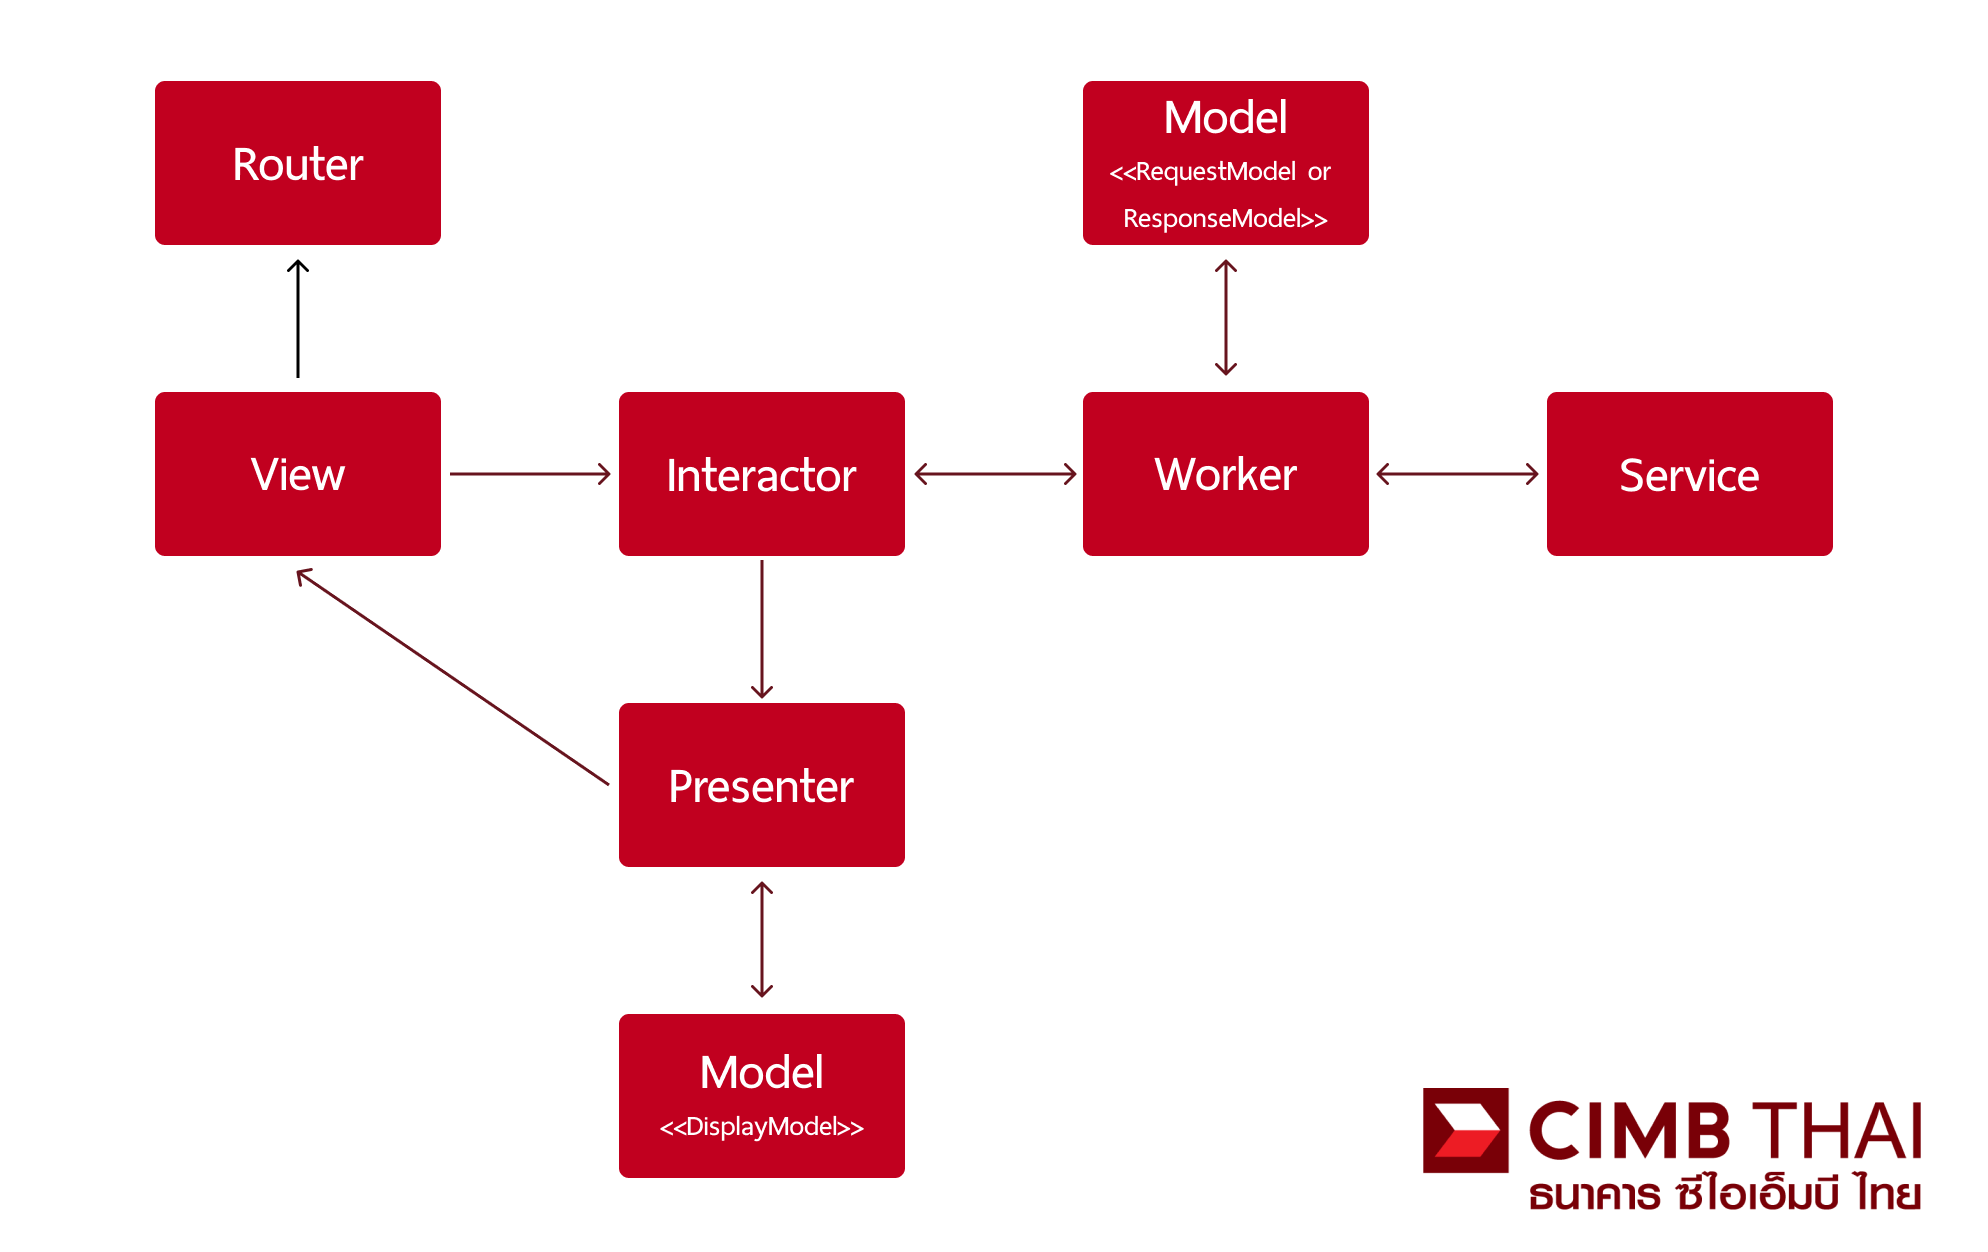
\includegraphics[width=1\textwidth]{vip-pattern}
            \caption{รูปแบบการทำงานของ VIP}\label{vip-pattern}
        \end{figure}
        VIP คือรูปแบบในการพัฒนาซอฟต์แวร์รูปแบบหนึ่งที่แบ่งแยกการแสดงผล และส่วน Business Logic ออกจากกันโดยแยกออกมาหลัก ๆ ได้ 3 ส่วนคือ View, Interactor และ Presenter แต่ว่าจะมีส่วนแยกออกมาเพื่อทำงานให้สมบูรณ์อีกคือ Model, Router และ Worker
        ซึ่งแต่ละส่วนนั้นทำงานดังนี้
        \begin{enumerate}
            \item \textbf{View} เป็นส่วนติดต่อลูกค้าที่จะคอยรับข้อมูลและแสดงผลให้ลูกค้า เมื่อมีข้อมูลเข้ามาจากลูกค้า Activity(Android) หรือ ViewController(iOS) เป็นคลาสที่คอยรับข้อมูลเพื่อส่งต่อให้ Interactor นำไปประมวลผลต่อ และแสดงผลโดยการนำข้อมูลที่จัดรูปแบบแล้วจาก Presenter มาแสดงผลให้กับลูกค้า
            \item \textbf{Interactor} เป็นส่วนที่คอยรับการสั่งการมาจาก View เพื่อจัดเตรียมข้อมูล หรือคำนวณข้อมูลเพื่อที่จะส่งต่อไปยัง Presenter โดยข้อมูลนั้นจะมาจาก Worker ที่เป็นตัวส่งข้อมูลมาให้ เป็นที่ ๆ เกิด Business Logic ทุกอย่างที่นี่
            \item \textbf{Worker} เป็นส่วนดึงข้อมูลจาก Service เพื่อนำมาใส่ Model ที่จัดเตรียมไว้เพื่ออยู่ในรูปแบบที่ใช้งานกับโค้ดทุก ๆ ส่วนในแอปพลิเคชันได้ หรือเป็นตัวสร้าง Request Model เพื่อร้องขอไปยัง Service
            \item \textbf{Model (Response/Request)} เป็น Model ที่จะมีโครงสร้างเหมือน JSON ที่ได้รับการตอบรับมาจาก Service เพื่อที่จะสามารถนำข่้อมูลมาใส่ได้
            \item \textbf{Service} เป็นส่วนที่ดึงข้อมูลจาก API เพื่อให้ได้การตอบรับแบบ JSON เพื่อที่จะส่งต่อไป Worker หรือนำข้อมูลที่ได้จาก Worker ส่งไปยัง API เพื่อร้องขอข้อมูล
            \item \textbf{Presenter} เป็นส่วนที่จะคอยนำข้อมูลจาก Interactor มาจัดในรูปแบบที่จะแสดงผล หรือคือ DisplayModel เพื่อที่จะส่งไปให้กับ View ได้แสดงผล
            \item \textbf{Model (Display)} เป็น Model ที่จะมีโครงสร้างตามลักษณะของส่วนติดต่อลูกค้า
            \item \textbf{Router} เป็นส่วนที่คอยจัดการเรื่องการพาไปยังส่วนติดต่อลูกค้าในหน้าอื่น ๆ
        \end{enumerate}

    \subsection{Continuous Integration/Continuous Delivery (CI/CD)}
    \textbf{Continuous Integration (CI)} คือ กระบวนท่าที่ใช้สำหรับการรวบรวมซอฟแวร์ที่มีการพัฒนาแยกส่วนกันอย่างอัตโนมัติ อาจจะโดยหนึ่งหรือหลายนักพัฒนาก็ตามที สุดท้ายแล้วซอฟแวร์ที่พัฒนาชิ้นเล็กๆ ที่พัฒนาขึ้นมาจะต้องนำมารวมกันเป็นชิ้นใหญ่หนึ่งชิ้น จะทำอย่างไรให้มั่นใจได้ว่า ไม่มีชิ้นส่วนใดที่จะส่งผลให้ชิ้นส่วนอื่นๆ พังเสียหาย เนื่องจากเป็นการพัฒนาโดยโปรแกรมเมอร์หลายคน
    ซึ่งเป็นไปได้ว่าจะมี bug หลุดมาจากส่วนใดส่วนหนึ่ง แล้วเราจะป้องกันได้อย่างไรละ ดังนั้นจึงต้องมีการเขียน script test ที่คอยทดสอบความเข้ากันได้ของแต่ละชิ้นส่วนโดยอัตโนมัตินั่นเอง โดยการ Testing จะเริ่มตั้งแต่ Unit Testing ซึ่งสร้างจากทีมพัฒนา และเป็นส่วนจะใช้ตรวจสอบว่าสิ่งที่ทีมพัฒนายังทำงานถูกต้องและจะใช้เวลาช่วงสั้น ๆ เท่านั้น
    โดยในโลกของการพัฒนานั้น มักใช้ Build Server มาช่วยเพื่อให้เป้าหมายที่ตั้งไว้สำเร็จ กล่าวคือ จะเริ่มทำการ Integration กันตั้งแต่เมื่อมีการเปลี่ยนแปลง Source Code ที่ Repository กลาง ระบบจะทำการตรวจสอบ Code หลังจากการเปลี่ยนแปลงว่าทำงานร่วมกันได้หรือไม่ตั้งแต่ Compile, Testing
    
    ส่วน \textbf{CD} นั้นสามารถแบ่งได้สองประเภทตามวิธีการ Deploy ดังรูปที่ \ref{cd}
    \begin{figure}[H]
        \centering
        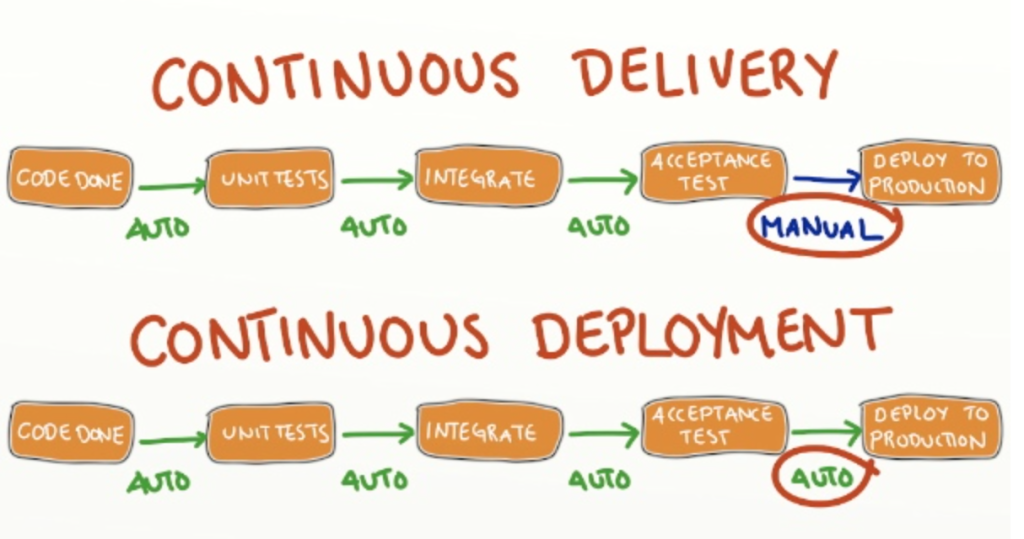
\includegraphics[width=1\textwidth]{cd}
        \caption{ความแตกต่างของ Continuous Deployment และ Continuous Delivery }\label{cd}
    \end{figure}
    \begin{itemize}
        \item[-] Continuous Deployment คือ ในทุกๆ ขั้นตอนจนถึงการ deployment ขึ้น production จะทำแบบอัตโนมัติทั้งหมด
        \item[-] Continuous Delivery คือ การงานต่างๆ ใน deployment pipeline นั้น จะเริ่มต้นทำงานตั้งแต่การ compile, build ไปจนถึงขั้นตอนการทดสอบต่างๆ เช่น Acceptance test เป็นแบบอัตโนมัติทั้งหมด ส่วนในขั้นตอนการ deployment ขึ้น production นั้น จะต้องได้รับการอนุมัติหรือการตัดสินใจกันก่อนจากทาง Business ซึ่งเป็นการทำงานแบบ manual นั่นเอง หรืออาจจะเป็น One Click Deploy ก็ได้\cite{cicd}
    \end{itemize}

\section{เครื่องมือที่ใช้งาน}
    \subsection{Android Studio}
        \begin{figure}[H]
            \centering
            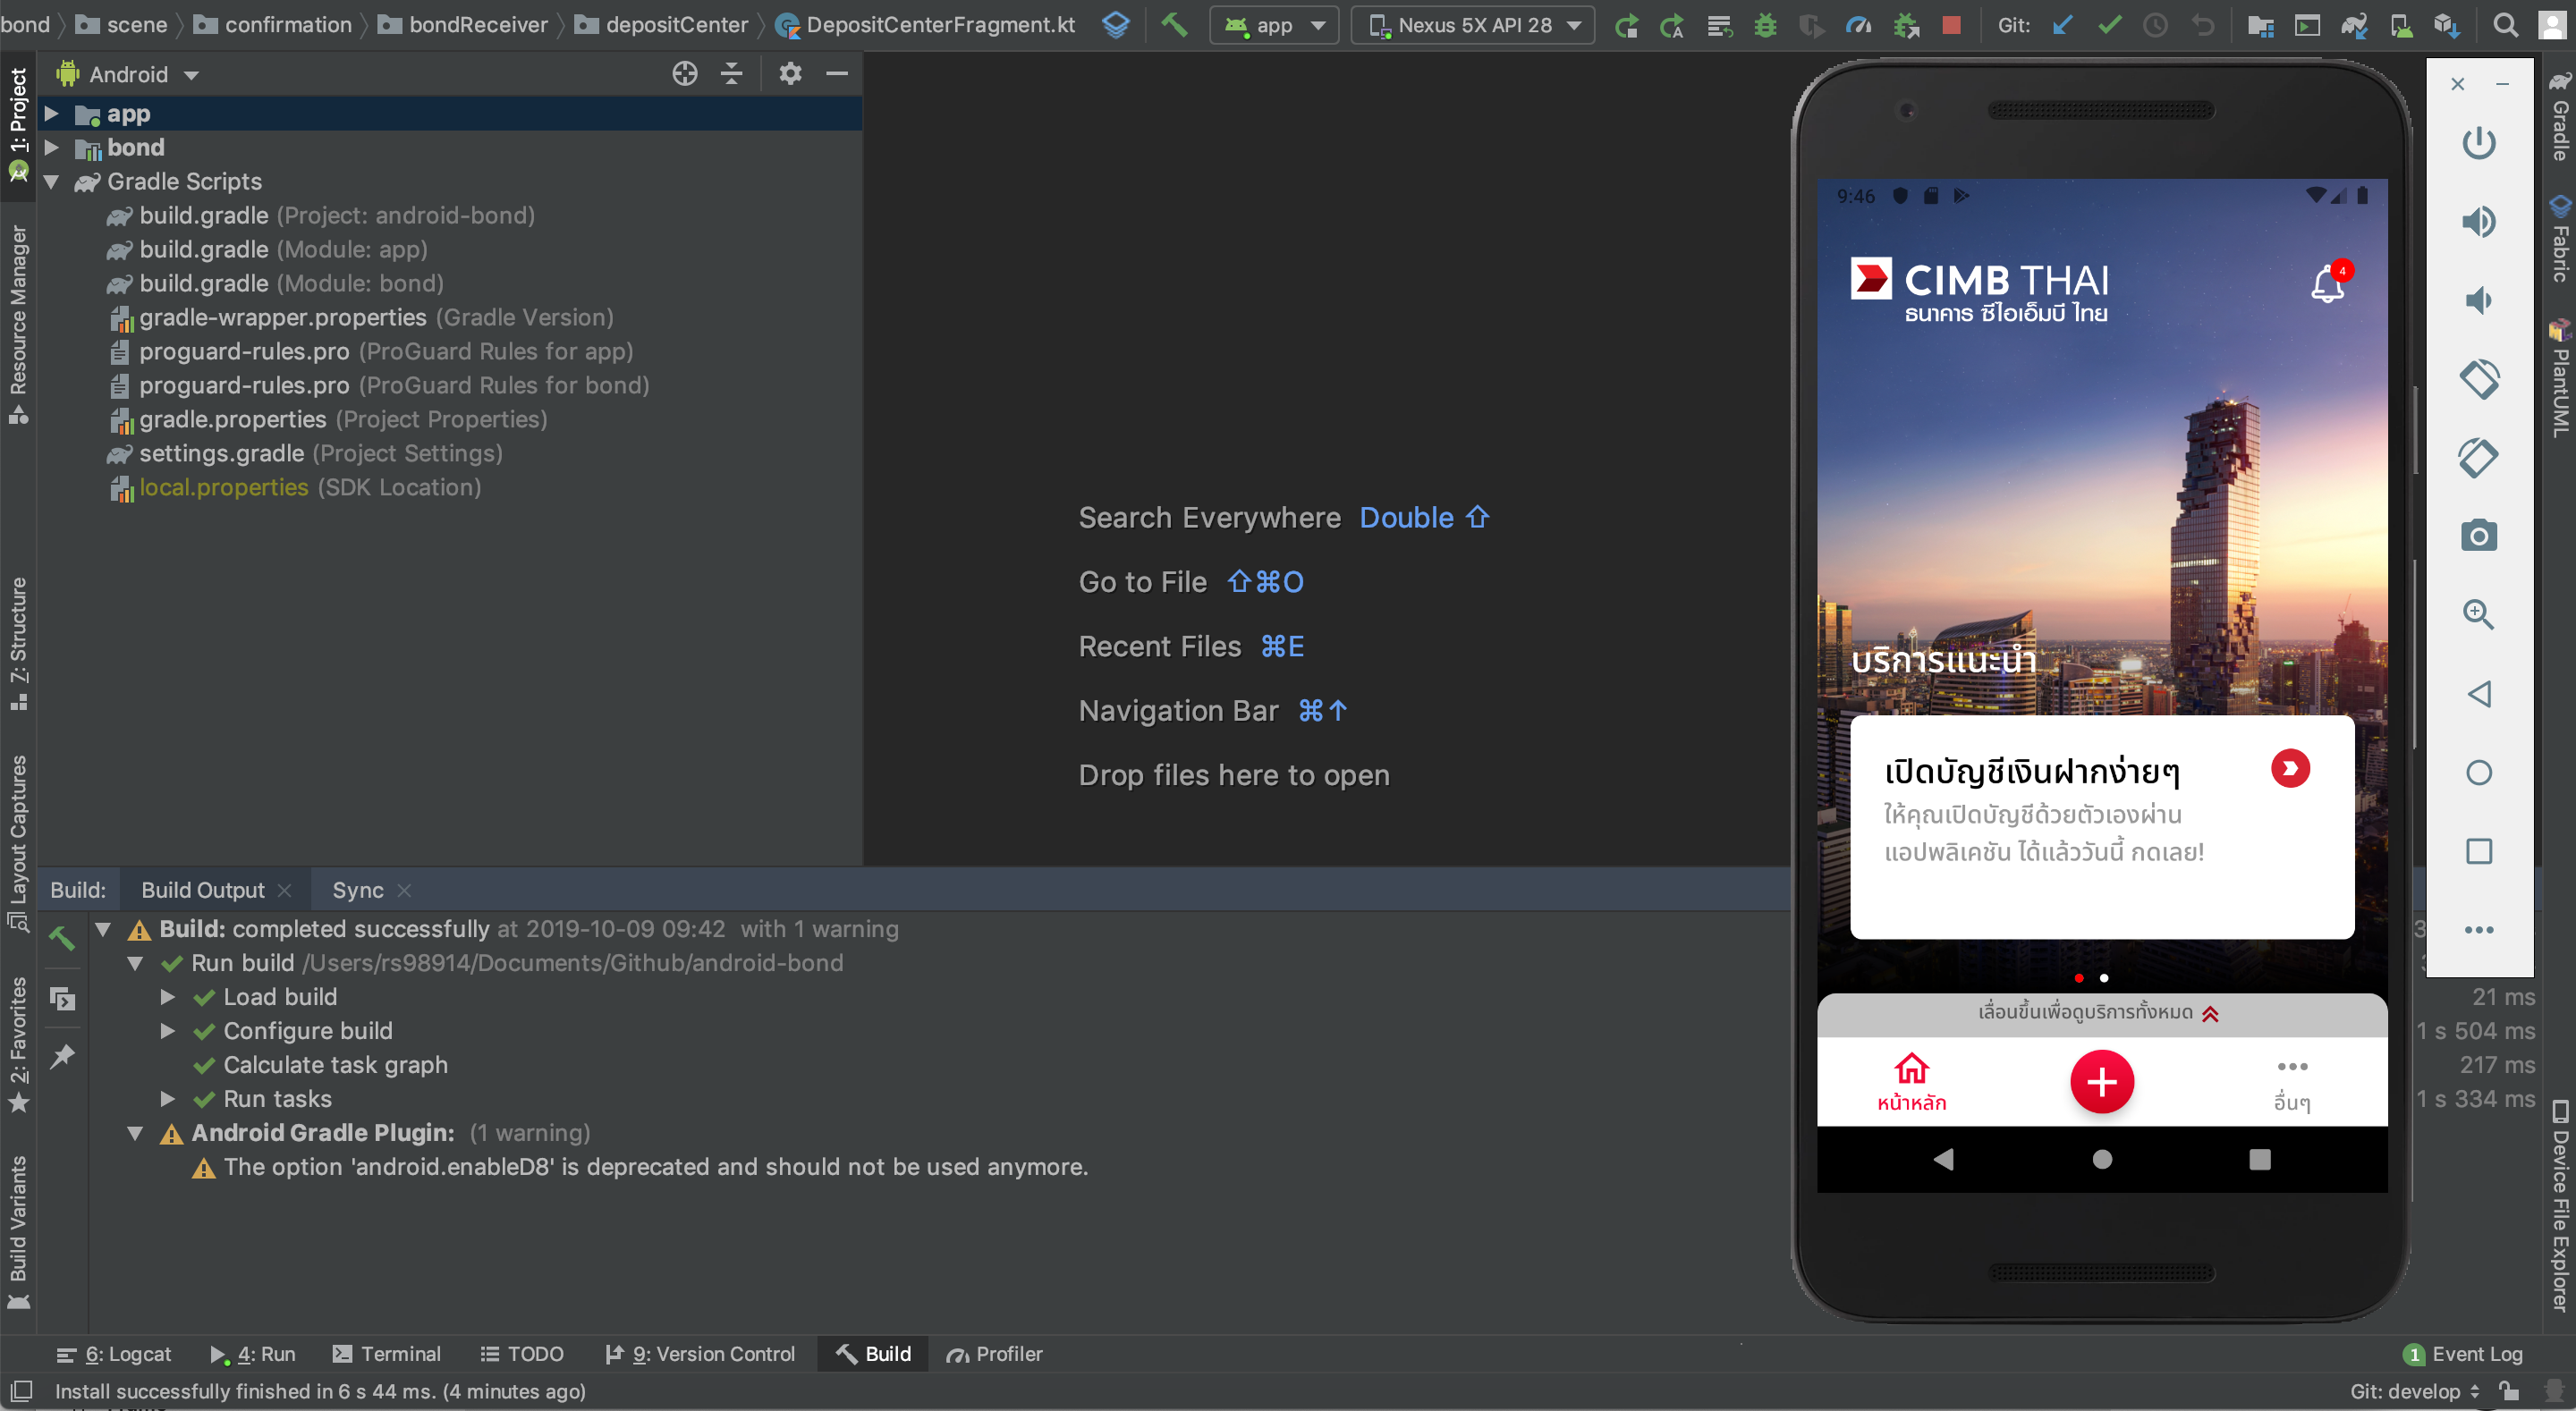
\includegraphics[width=1\textwidth]{android-studio}
            \caption{หน้าการใช้งาน Android Studio}\label{android-studio}
        \end{figure}
        Android Studio คือเครื่องมือพัฒนา IDE (ไอ ดี อี) หรือ Integrated Development Environment (อินทิเกรต ดีเวลลอปเม้นท์ (เอนไวรอนเม้นท์) ที่ถูกสร้างขึ้นมาเพื่อการพัฒนาแอนดรอยด์แอปพลิเคชั่น บนพื้นฐานของแนวคิด InteliJ IDEA(อินเทล ไอ เจ ไอดีอีเอ) คล้าย ๆ กับการทำงานของ Eclipse (อีคิปส์)และ Android ADT Plugin (แอนดรอยด์ เอดีที ปลั๊กอิน) และเป็น IDE Tools (ไอ ดี เอ็ม ทูล) ล่าสุดจาก Google (กูเกิ้ล)  ไว้พัฒนาโปรแกรม Android (แอนดรอยด์)\cite{android-studio}

    \subsection{Kotlin}
        \begin{figure}[H]
            \centering
            
\includegraphics[width=0.5\textwidth]{kotlin-logo}
            \caption{ตราสัญลักษณ์ภาษา Kotlin}\label{kotlin-logo}
        \end{figure}
        Kotlin คือภาษาโปรแกรมมิ่งที่ได้รวมหลักการเขียนโปรแกรมแบบเชิงวัตถุ และ หลักการเขียนโปรแกรมแบบฟังก์ชันเข้ามาร่วมกันซึ่งยังคงทำงานกับ JVM เช่นเดียวกับ Java แต่ได้เพิ่มความสามารถใหม่ที่ไม่มีใน Java และแก้ไขข้อผิดพลาดที่เกิดขึ้นใน Java รวมทั้ง Syntax ก็สั้นกระชับเข้าใจง่ายและมีความปลอดภัยสูง  เพราะ Kotlin จะเข้มงวดกับการประกาศประเภทของตัวแปรอย่างมาก โดยภาษา Kotlin ถูกพัฒนาโดยบริษัท JetBrains

    \subsection{Xcode}
        \begin{figure}[H]
            \centering
            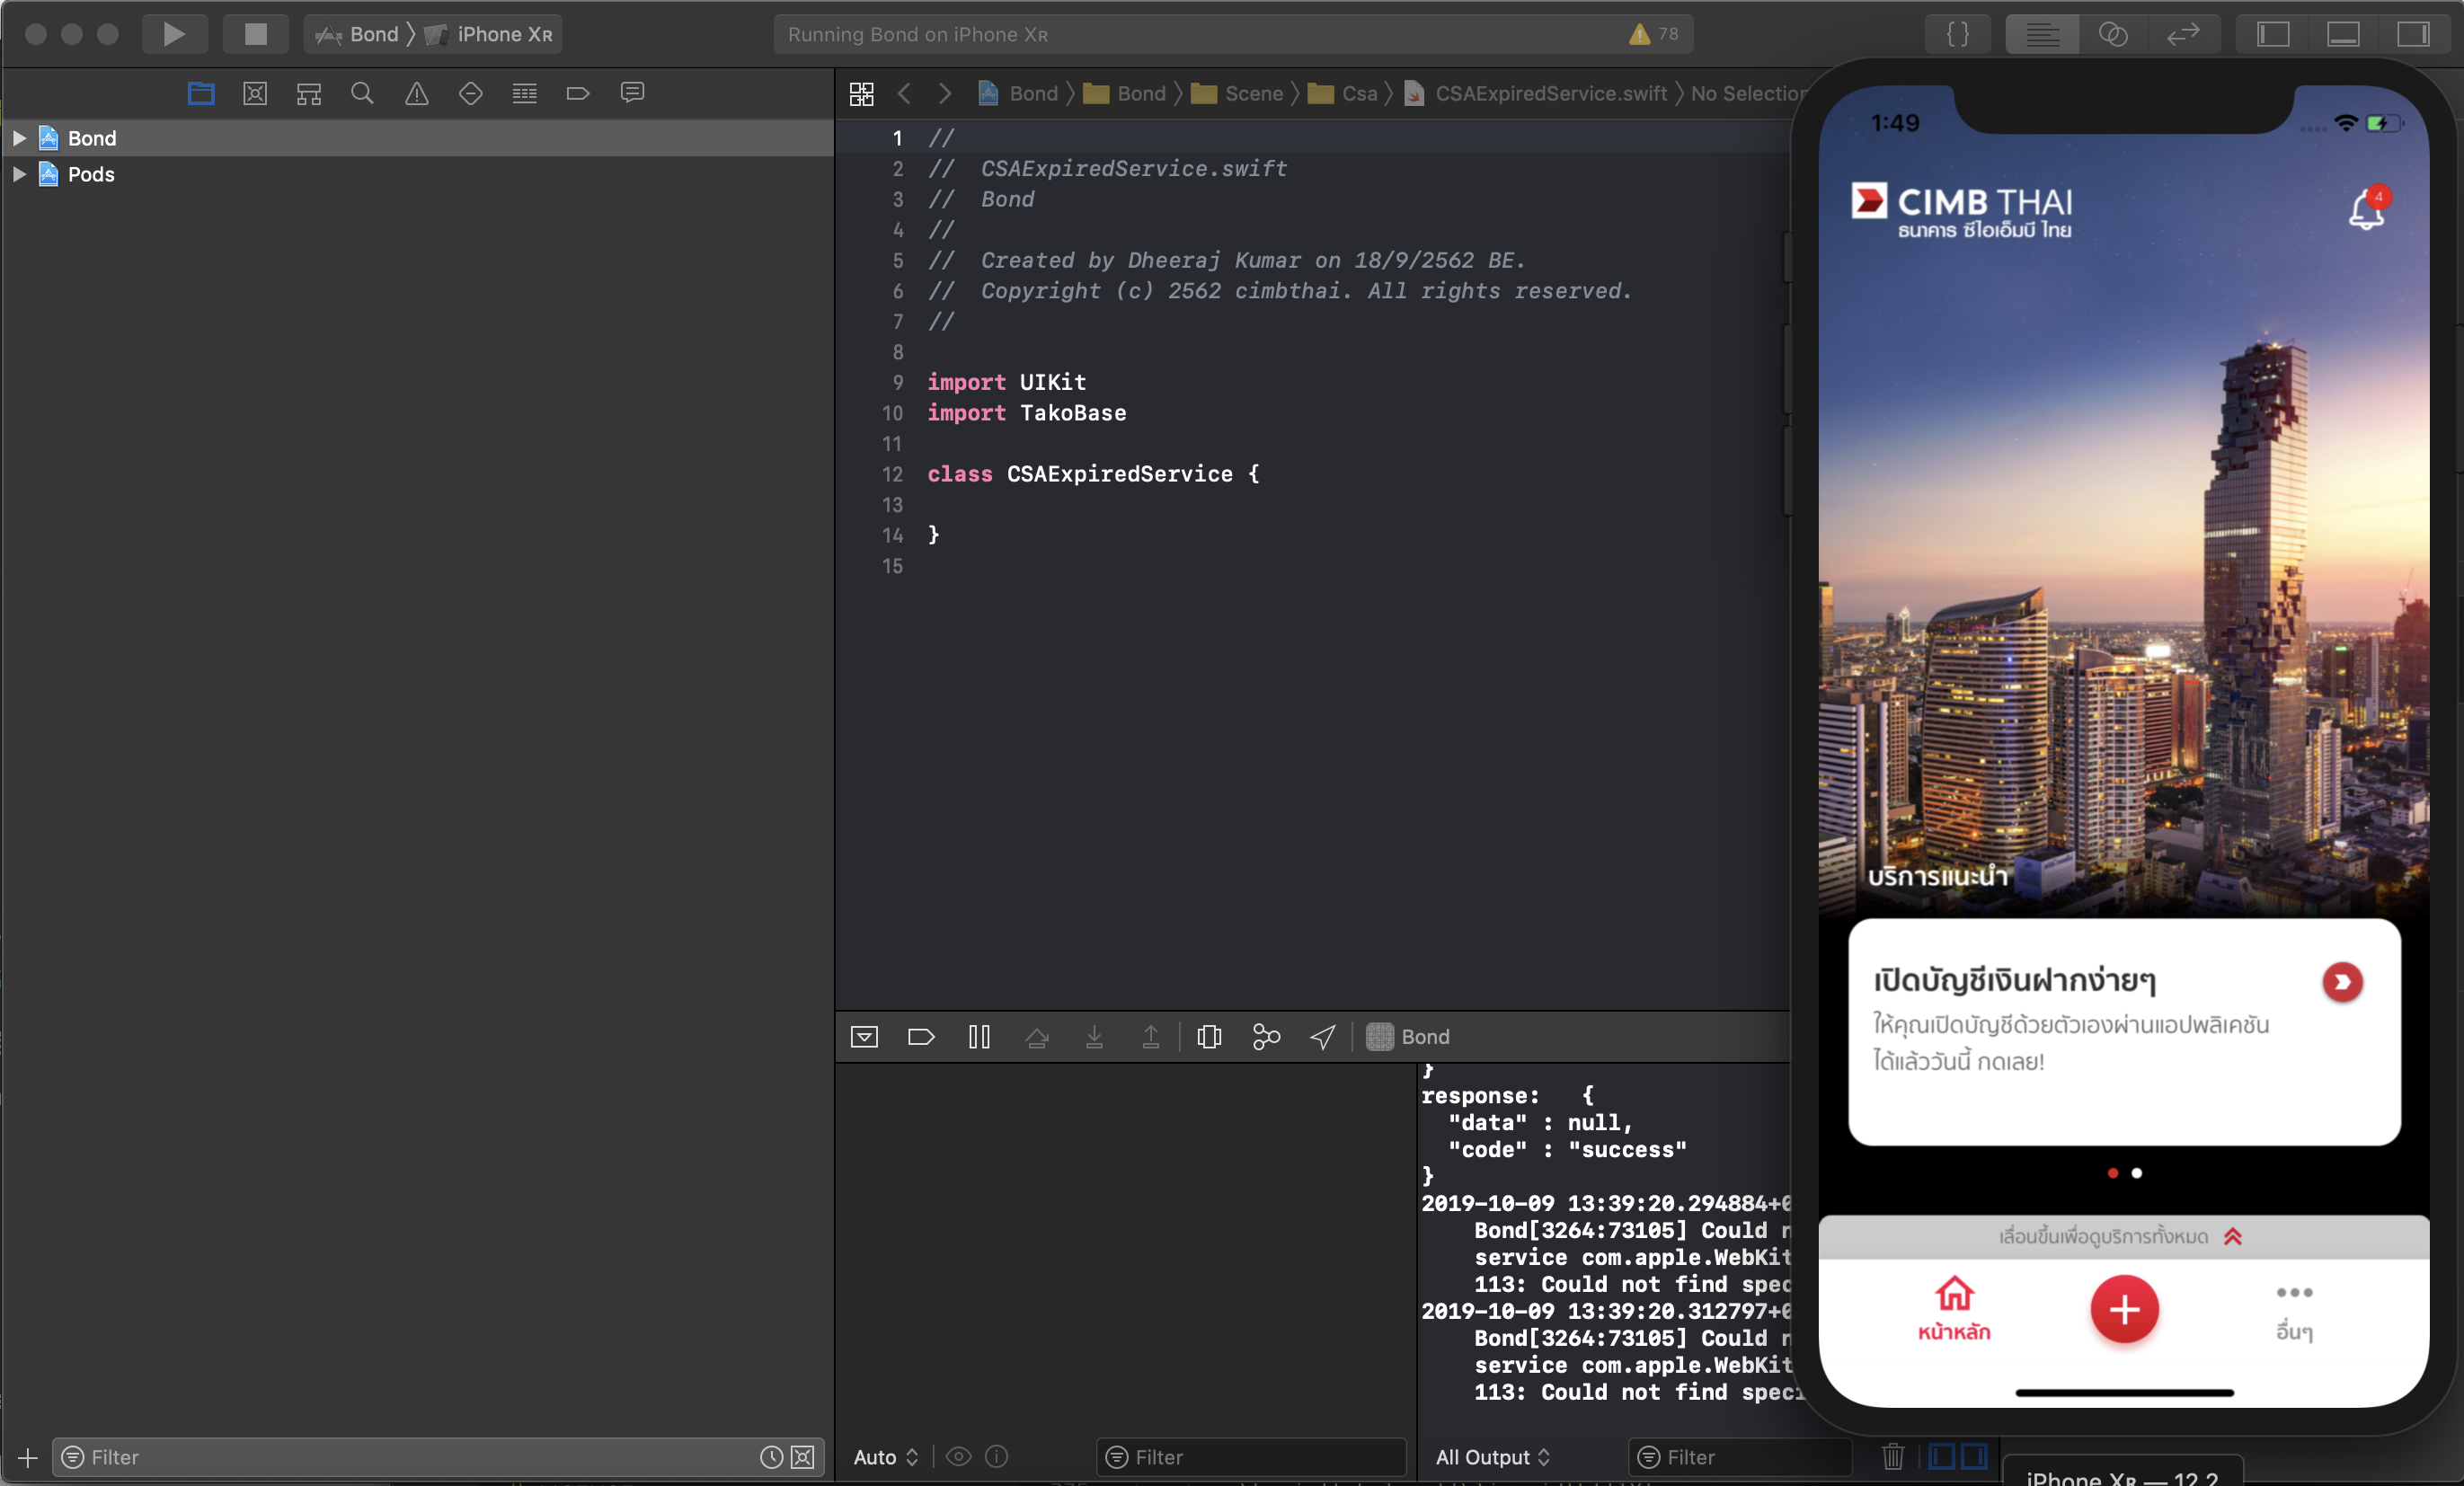
\includegraphics[width=1\textwidth]{xcode}
            \caption{หน้าการใช้งาน Xcode}\label{xcode}
        \end{figure}
        Xcode คือเครื่องมือสำหรับนักพัฒนาโปรแกรม และแอปพลิเคชันบนแพลตฟอร์ม OS X และ iOS บนสมาร์ทโฟนที่ผลิตโดยบริษัท Apple

    \subsection{Swift}
        \begin{figure}[H]
            \centering
            
\includegraphics[width=0.5\textwidth]{swift-logo}
            \caption{ตราสัญลักษณ์ภาษา Swift}\label{swift-logo}
        \end{figure}
        Swift คือภาษาโปรแกรมที่บริษัท Apple ได้สร้างและออกแบบมาเพื่อให้นักพัฒนาใช้พัฒนาโปรแกรมบน Mac OS X และ iOS โดยในอดีตจนถึงปัจจุบันภาษาที่ใช้คือ Objective-C โดยSwift เป็นภาษาที่ออกแบบให้มีประสิทธิภาพสูงและง่ายต่อการพัฒนาโดยนำข้อดีของภาษาสมัยใหม่เข้ามามากมาย เช่น Type Inference, Clean Syntax, No semicolons, Closures, Generics ซึ่งคุณสมบติที่กล่าวมาบางอย่างก็มีอยู่แล้วในภาษา Objective-C แต่ใน Swift นั้นจะน่าคบหามากขึ้น ภาษา Swift ยังถูกออกแบบให้มีความปลอดภัยในการเขียนโปรแกรมมากขึ้น\cite{swift}

    \subsection{IntelliJ IDEA CE}
        \begin{figure}[H]
            \centering
            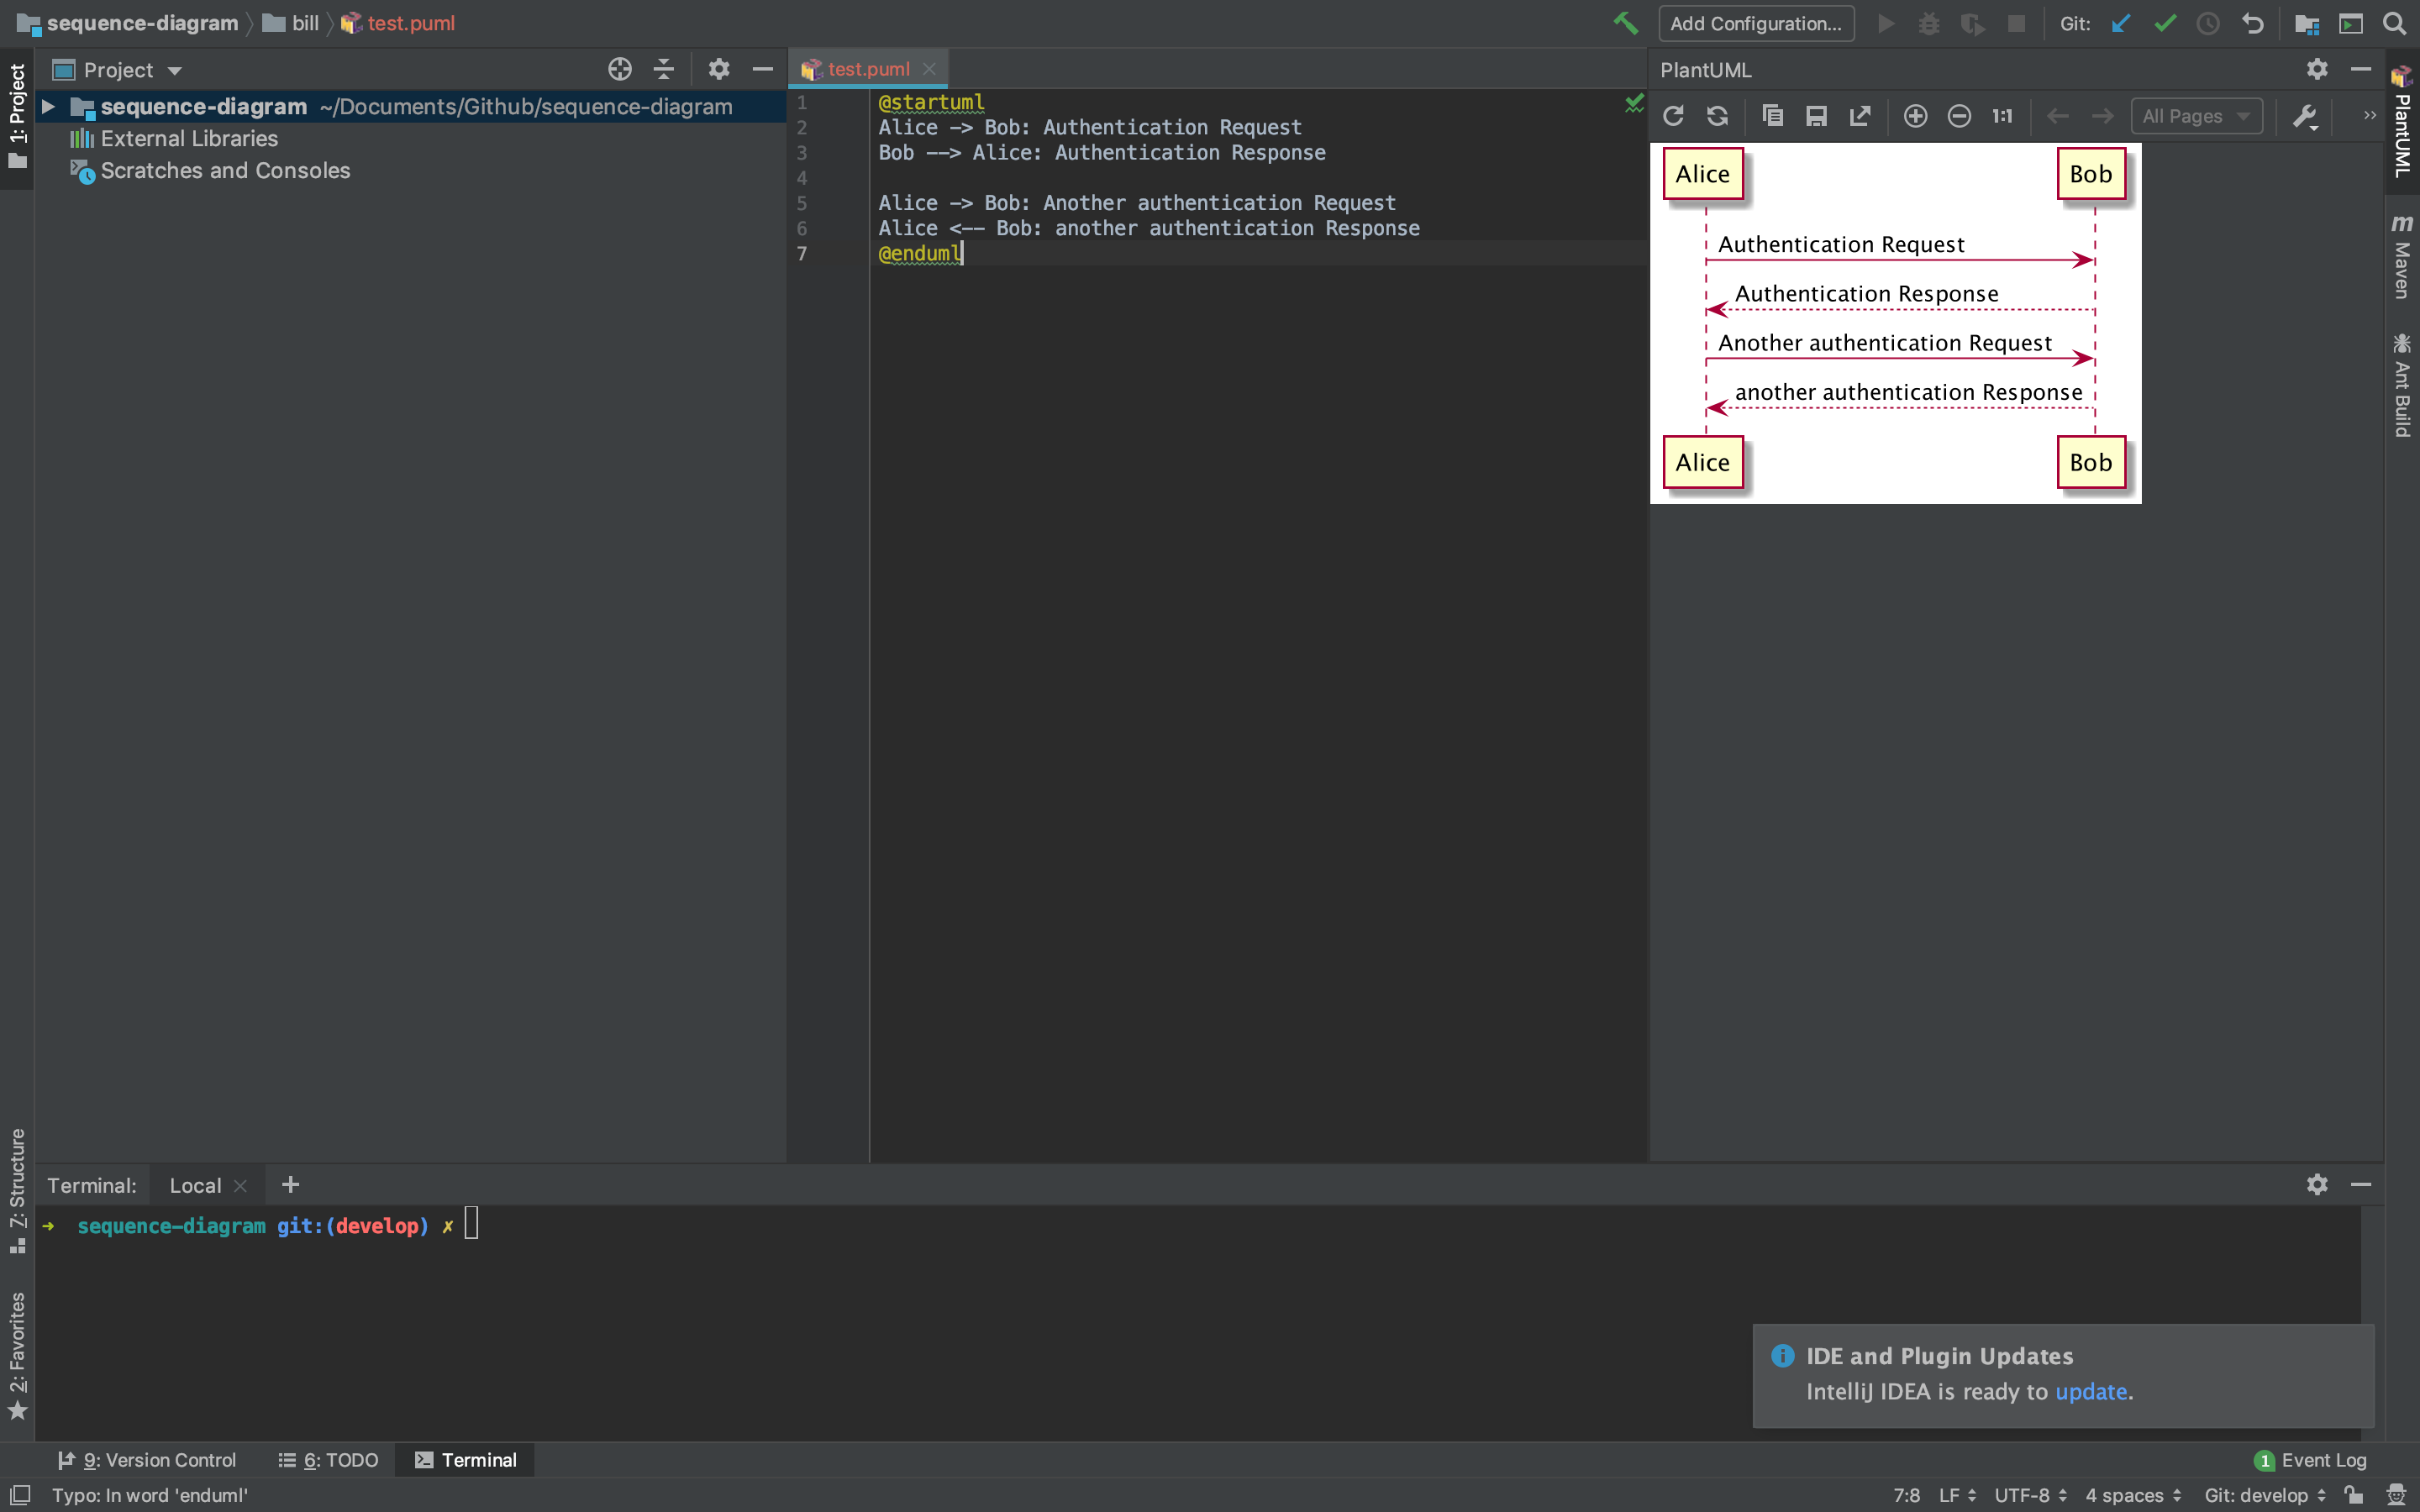
\includegraphics[width=1\textwidth]{intellij-idea}
            \caption{หน้าการใช้งาน IntelliJ IDEA CE}\label{intellij-idea}
        \end{figure}
        IntelliJ IDEA CE คือเครื่องมือที่ช่วยในการพัฒนาโปรแกรมที่พื้นฐานการทำงานเพื่อภาษา Java ที่ถูกพัฒนาโดยบริษัท JetBrains ซึ่งมีสิ่งอำนวยความสะดวกต่างๆ เช่น คำสั่ง Compile, Run และจัด Format Code อัตโนมัติเป็นต้น

    \subsection{Visual Studio Code}
        \begin{figure}[H]
            \centering
            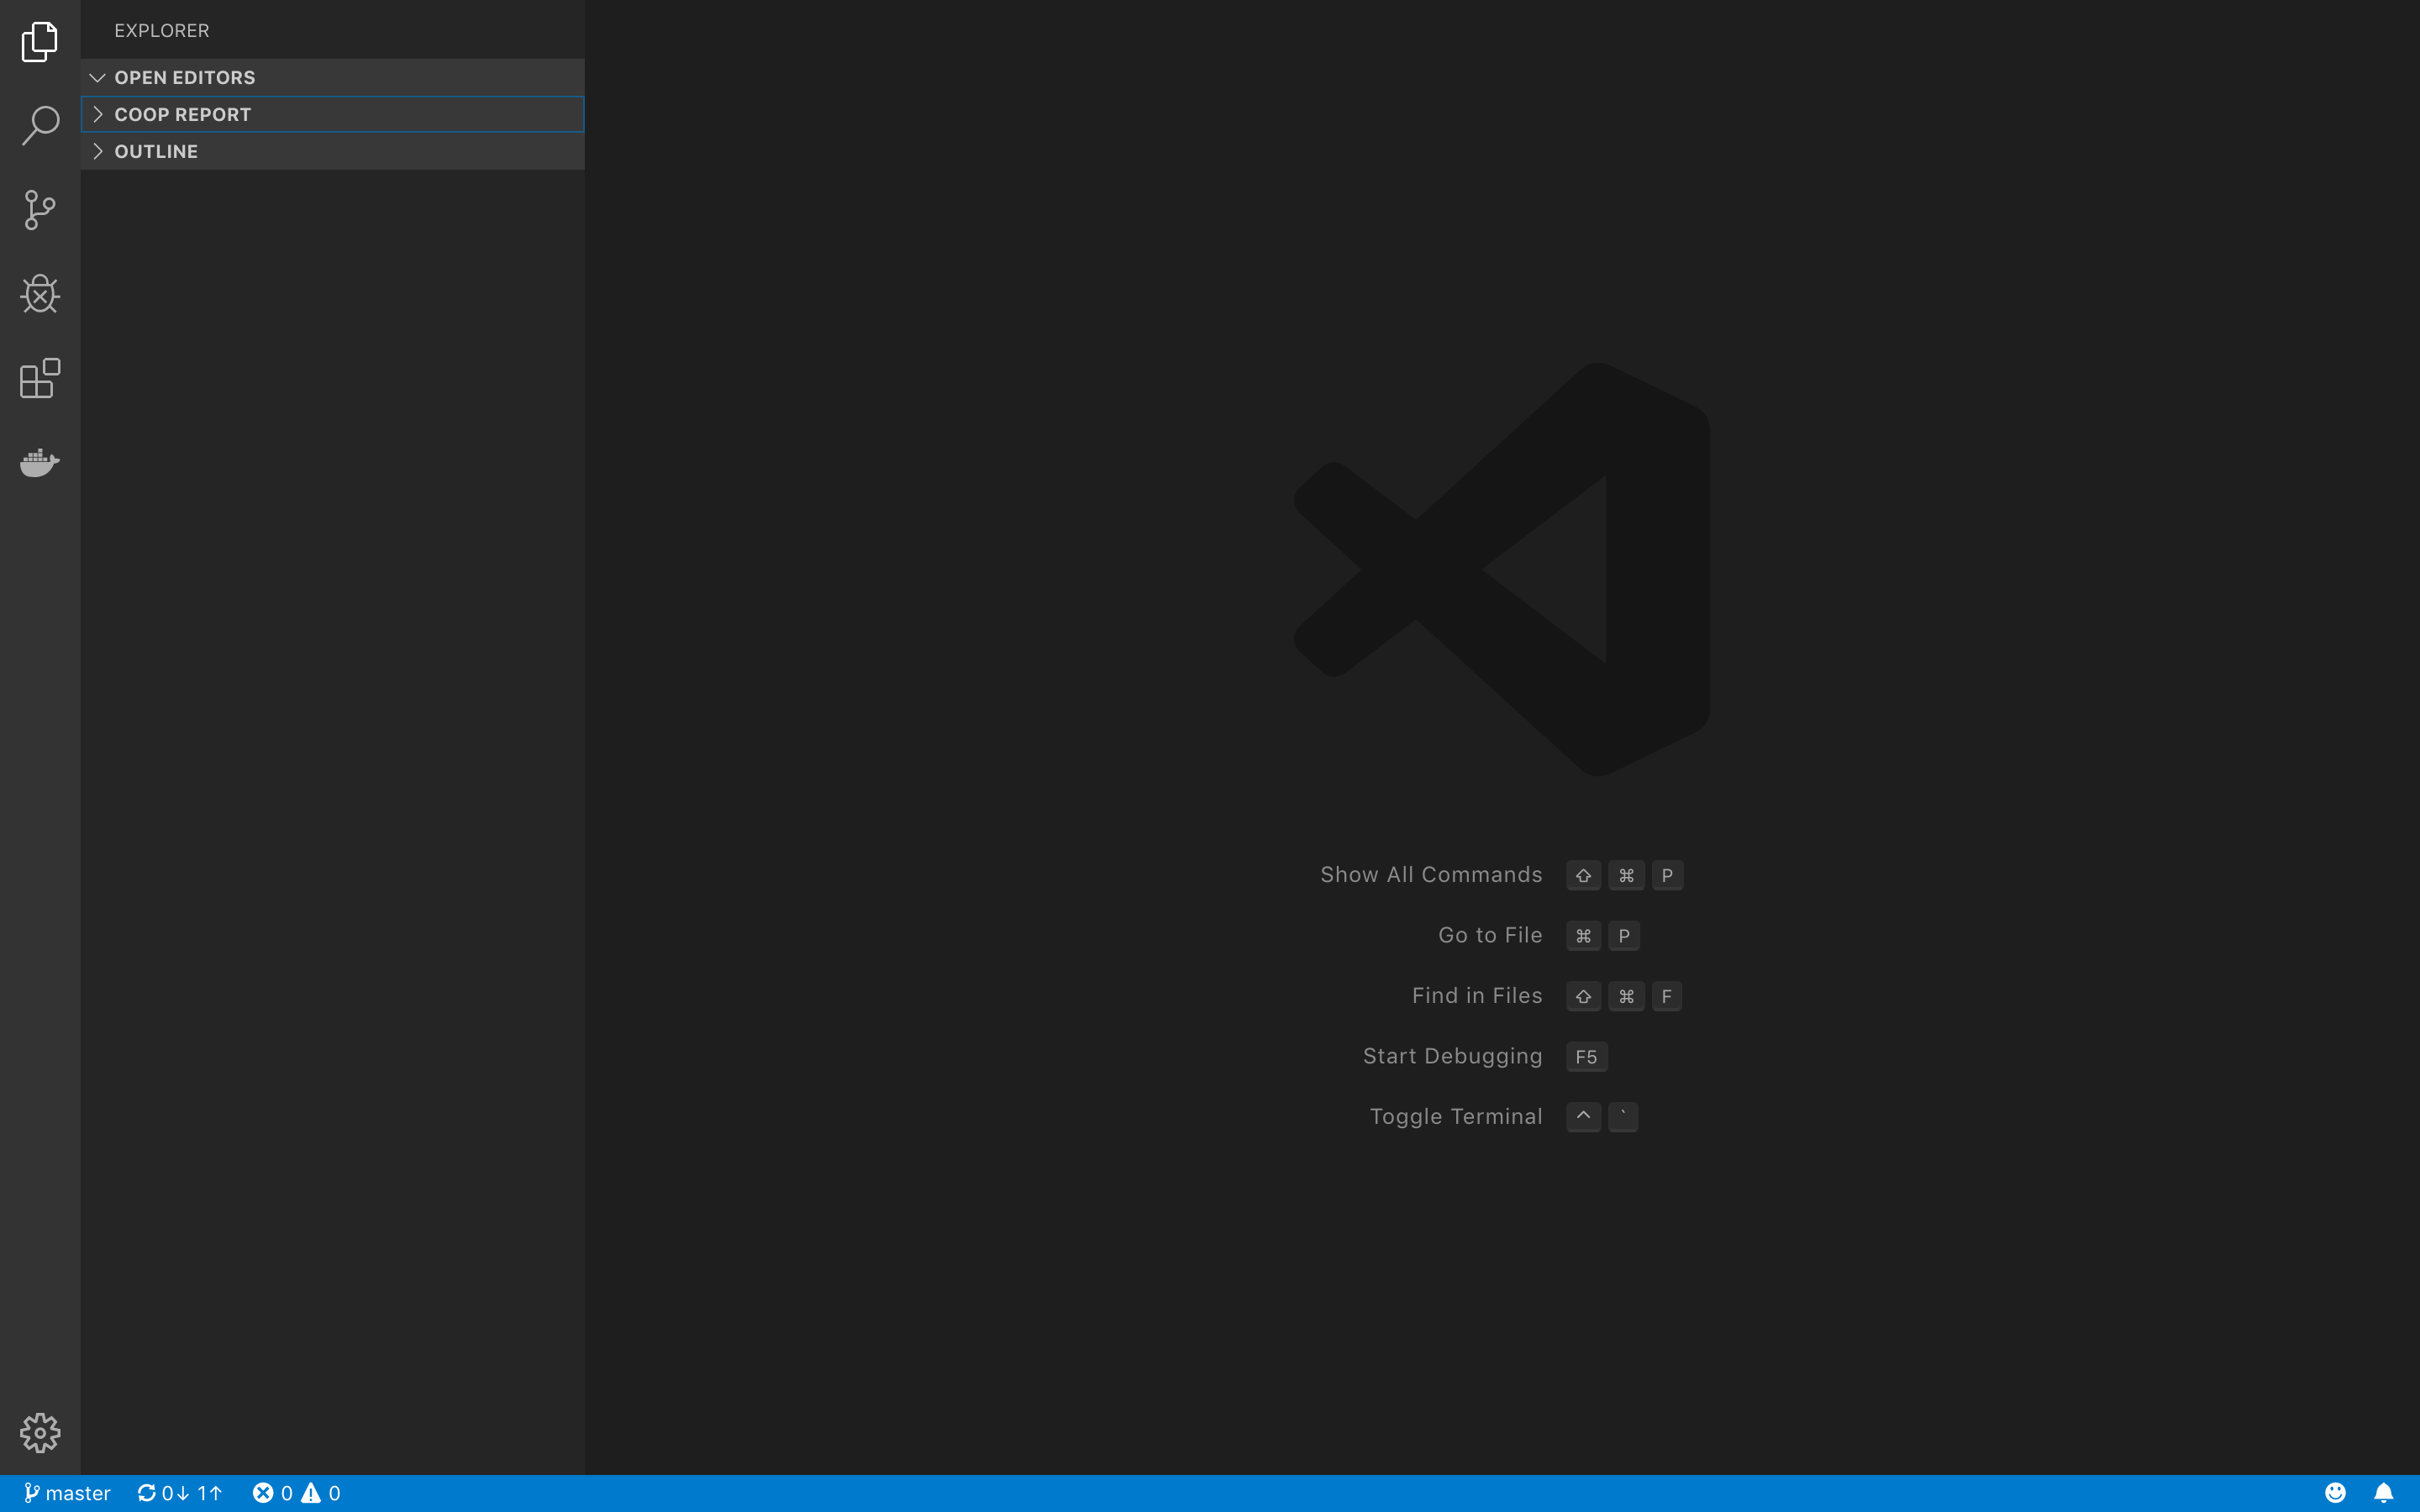
\includegraphics[width=1\textwidth]{visual-studio-code}
            \caption{หน้าการใช้งาน Visual Studio Code}\label{visual-studio-code}
        \end{figure}
        Visual Studio คือโปรแกรม Code Editor ที่ใช้ในการแก้ไขและปรับแต่งโค้ด จากค่ายไมโครซอฟท์ มีการพัฒนาออกมาในรูปแบบของ OpenSource จึงสามารถนำมาใช้งานได้แบบฟรี ๆ ที่ต้องการความเป็นมืออาชีพ
        ซึ่ง Visual Studio Code นั้น เหมาะสำหรับนักพัฒนาโปรแกรมที่ต้องการใช้งานข้ามแพลตฟอร์ม รองรับการใช้งานทั้งบน Windows, macOS และ Linux สนับสนุนทั้งภาษา JavaScript, TypeScript และ Node.js 
        สามารถเชื่อมต่อกับ Git ได้ นำมาใช้งานได้ง่ายไม่ซับซ้อน มีเครื่องมือส่วนขยายต่าง ๆ ให้เลือกใช้อย่างมากมาก

    \newpage
    \subsection{Python}
        \begin{figure}[H]
            \centering
            
\includegraphics[width=0.5\textwidth]{python-logo}
            \caption{ตราสัญลักษณ์ภาษา Python}\label{python-logo}
        \end{figure}
        Python คือภาษาโปรแกรมคอมพิวเตอร์ระดับสูง โดยถูกออกแบบมาให้เป็นภาษาสคริปต์ที่อ่านง่าย  โดยตัดความซับซ้อนของโครงสร้างและไวยกรณ์ของภาษาออกไป ในส่วนของการแปลงชุดคำสั่งที่เราเขียนให้เป็นภาษาเครื่อง Python มีการทำงานแบบ Interpreter คือเป็นการแปลชุดคำสั่งทีละบรรทัด เพื่อป้อนเข้าสู่หน่วยประมวลผลให้คอมพิวเตอร์ทำงานตามที่เราต้องการ นอกจากนั้นภาษาโปรแกรม Python ยังสามารถนำไปใช้ในการเขียนโปรแกรมได้หลากหลายประเภท โดยไม่ได้จำกัดอยู่ที่งานเฉพาะทางใดทางหนึ่ง (General-purpose language) จึงทำให้มีการนำไปใช้กันแพร่หลายในหลายองค์กรใหญ่ระดับโลก

    \subsection{Django}
        \begin{figure}[H]
            \centering
            
\includegraphics[width=0.5\textwidth]{django-logo}
            \caption{ตราสัญลักษณ์ภาษา Django}\label{django-logo}
        \end{figure}
        Python คือเป็นโครงร่าง Python Web ระดับสูงที่สนับสนุนการพัฒนาอย่างรวดเร็วและการออกแบบที่สะอาดและใช้งานได้จริง สร้างขึ้นโดยนักพัฒนาที่มีประสบการณ์ดูแลความยุ่งยากในการพัฒนาเว็บไซต์เป็นอย่างมากดังนั้นคุณจึงสามารถมุ่งเน้นไปที่การเขียนแอพของคุณโดยไม่จำเป็นต้องคิดค้นใหม่

    \subsection{Vue.js}
        \begin{figure}[H]
            \centering
            
\includegraphics[width=0.5\textwidth]{vue-logo}
            \caption{ตราสัญลักษณ์ภาษา Vue.js}\label{vue-logo}
        \end{figure}
        Vue.js คือเป็น Progressive framework รูปแบบที่ถูกออกแบบมาให้จัดการ กับ UI โดยตัวหน้าที่หลักจะเน้นไปที่ส่วน View Layer เท่านั้น ด้วยการออกแบบที่ใช้งานได้ง่ายทำให้เหมาะสมกับการนำมาใช้ที่ส่วนๆ นึงใน Website หรือใช้กับทั้ง Website ได้เลยในรูปแบบของ Single Page Applcation 

    \subsection{Git}
        \begin{figure}[H]
            \centering
            
\includegraphics[width=0.5\textwidth]{git-logo}
            \caption{ตราสัญลักษณ์ Git}\label{git-logo}
        \end{figure}
        Git คือ Version Control แบบ Distributed ตัวหนึ่ง เป็นระบบที่ใช้จัดเก็บและควบคุมการเปลี่ยนแปลงที่เกิดขึ้นกับไฟล์ชนิดใดก็ได้ ไม่ว่าจะเป็น Text File หรือ Binary File (จากนี้จะขอเรียก Text File หรือ Binary File รวมกันว่า Source Code)

    \subsection{Hangouts Chat}
        \begin{figure}[H]
            \centering
            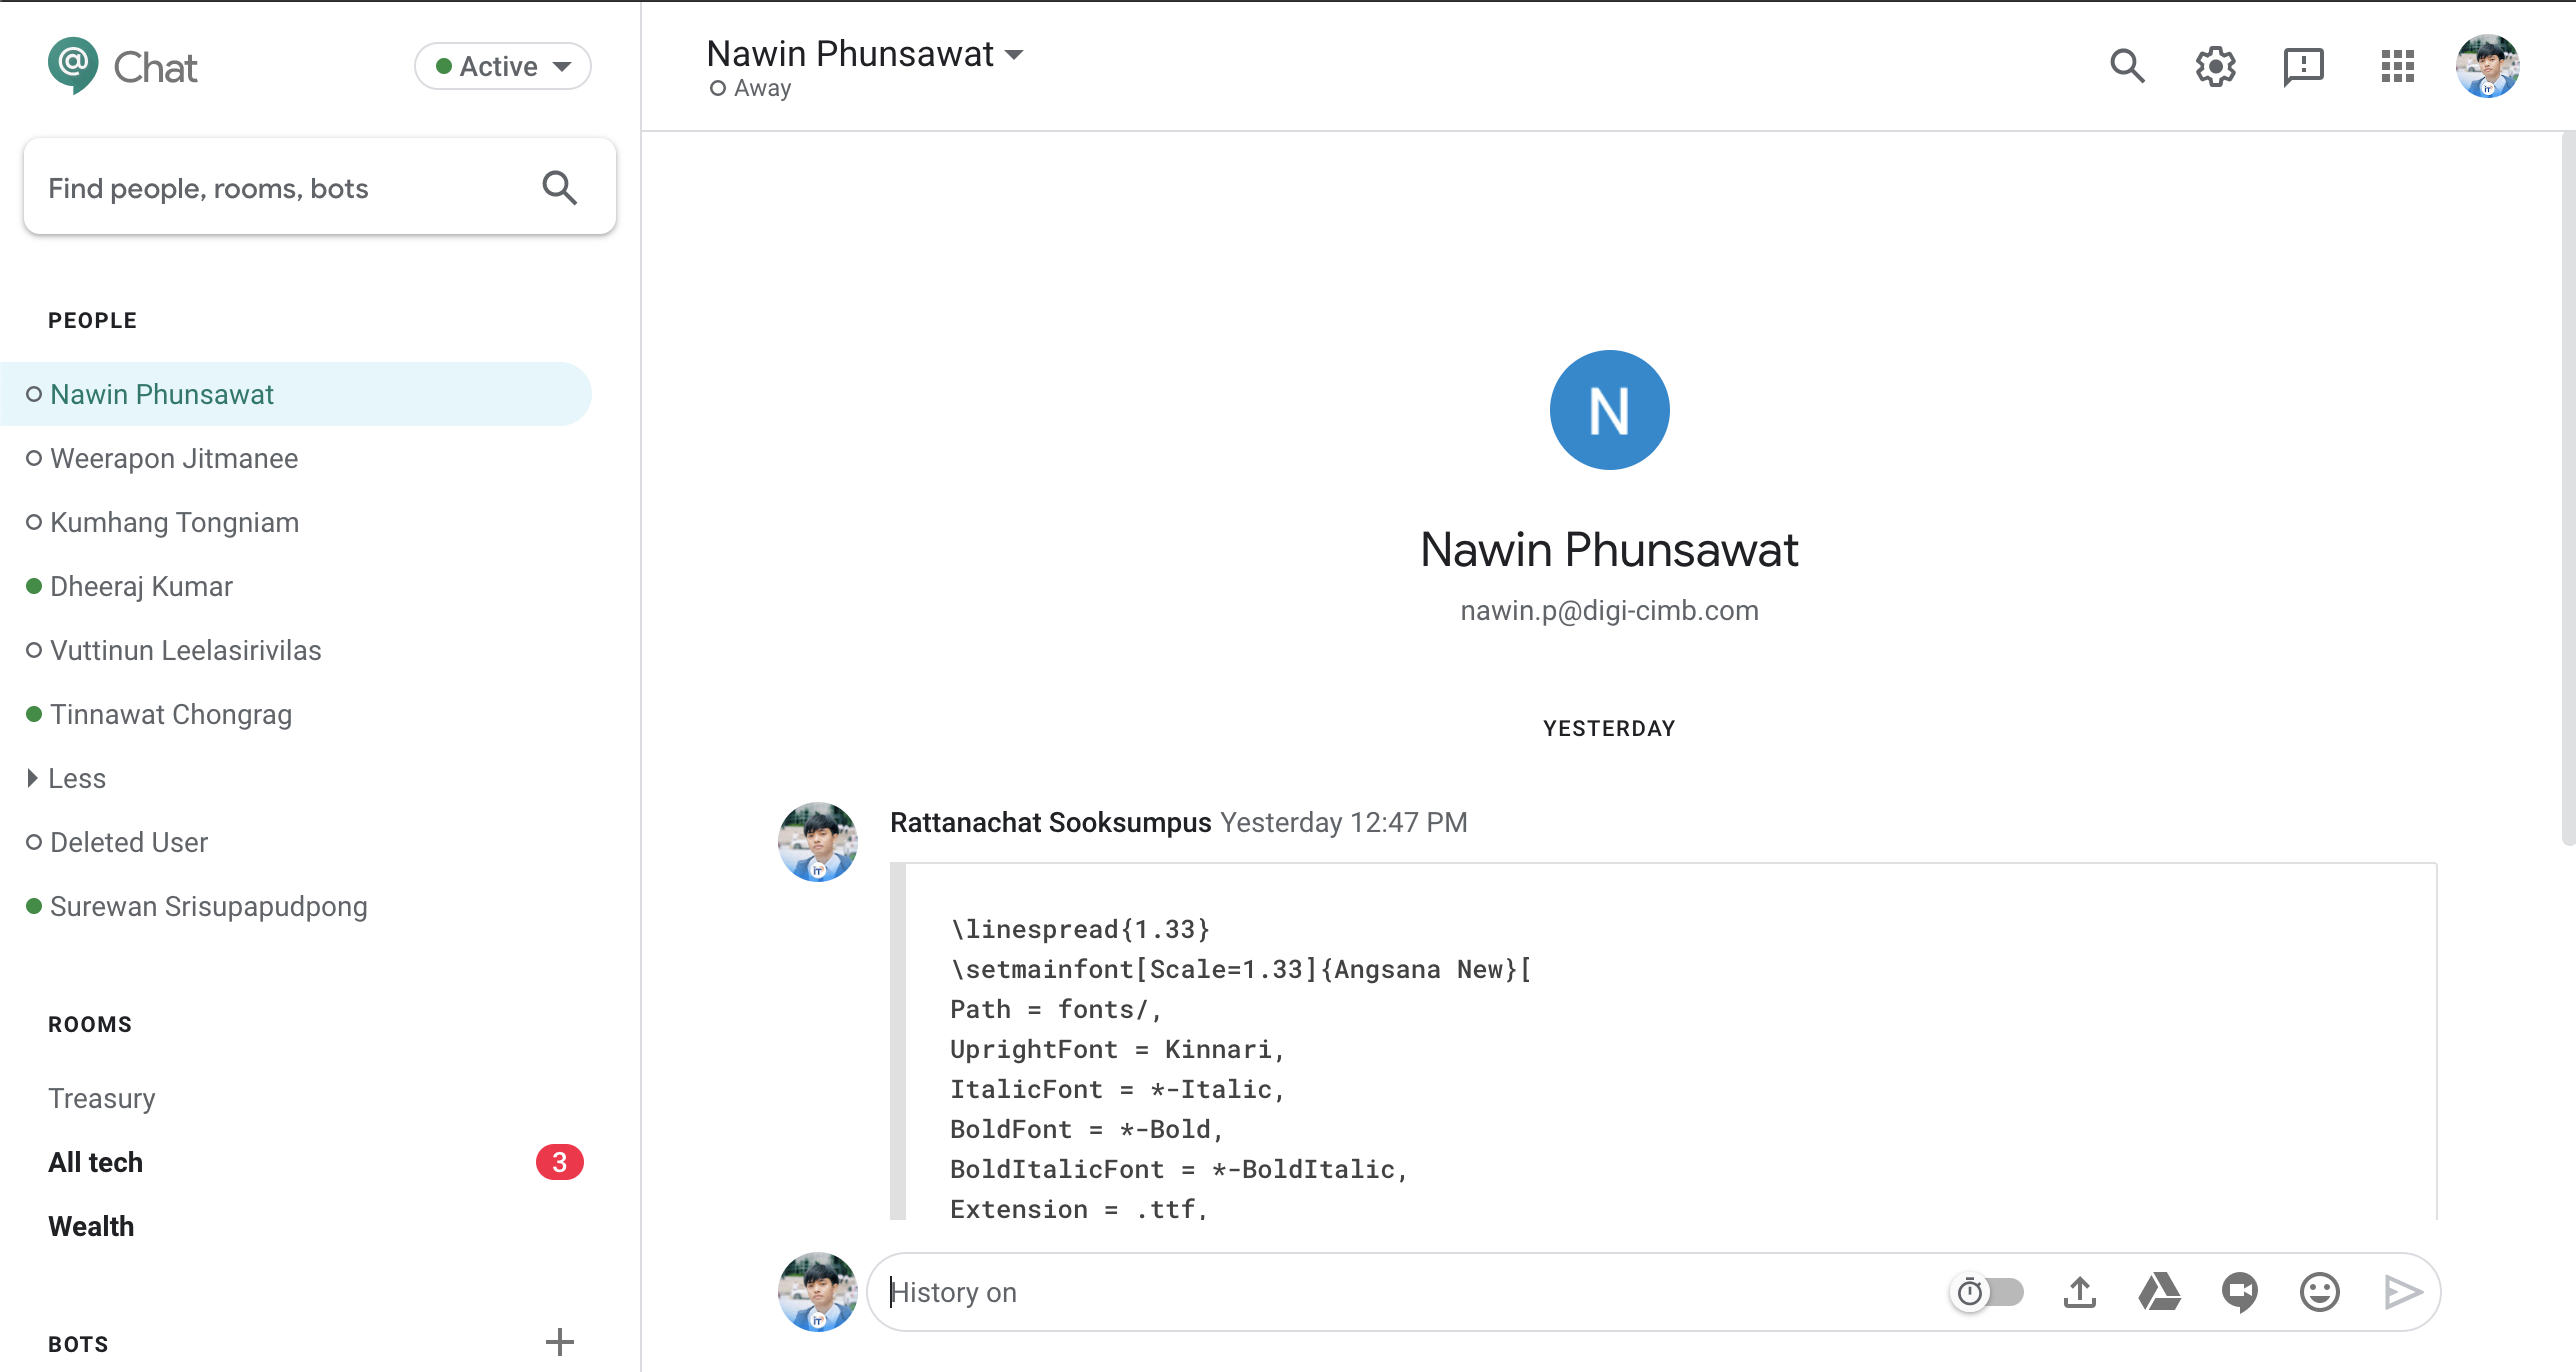
\includegraphics[width=1\textwidth]{chat}
            \caption{หน้าการใช้งาน Hangouts Chat}\label{chat}
        \end{figure}
        Hangouts Chat คือแพลตฟอร์มการรับส่งข้อความที่สร้างขึ้นสำหรับทีม ทำให้ทีมทำงานได้ง่ายขึ้น ไม่ว่าจะเป็นการส่งข้อความส่วนตัวหรือข้อความกลุ่ม ช่วยให้ทีมทำงานร่วมกันได้อย่างคล่องตัวและมีประสิทธิภาพ อีกทั้งยังติดตามความคืบหน้าและผลการทำงานได้ง่ายด้วยห้องแชทออนไลน์เพื่อการทำงานร่วมกันและการสนทนาแบบเป็นชุดข้อความ ตอนนี้ Chat รองรับทั้งหมด 28 ภาษา ห้องแชทแต่ละห้องรองรับสมาชิกได้สูงสุด 8,000 คน

    \subsection{Jira Software}
        \begin{figure}[H]
            \centering
            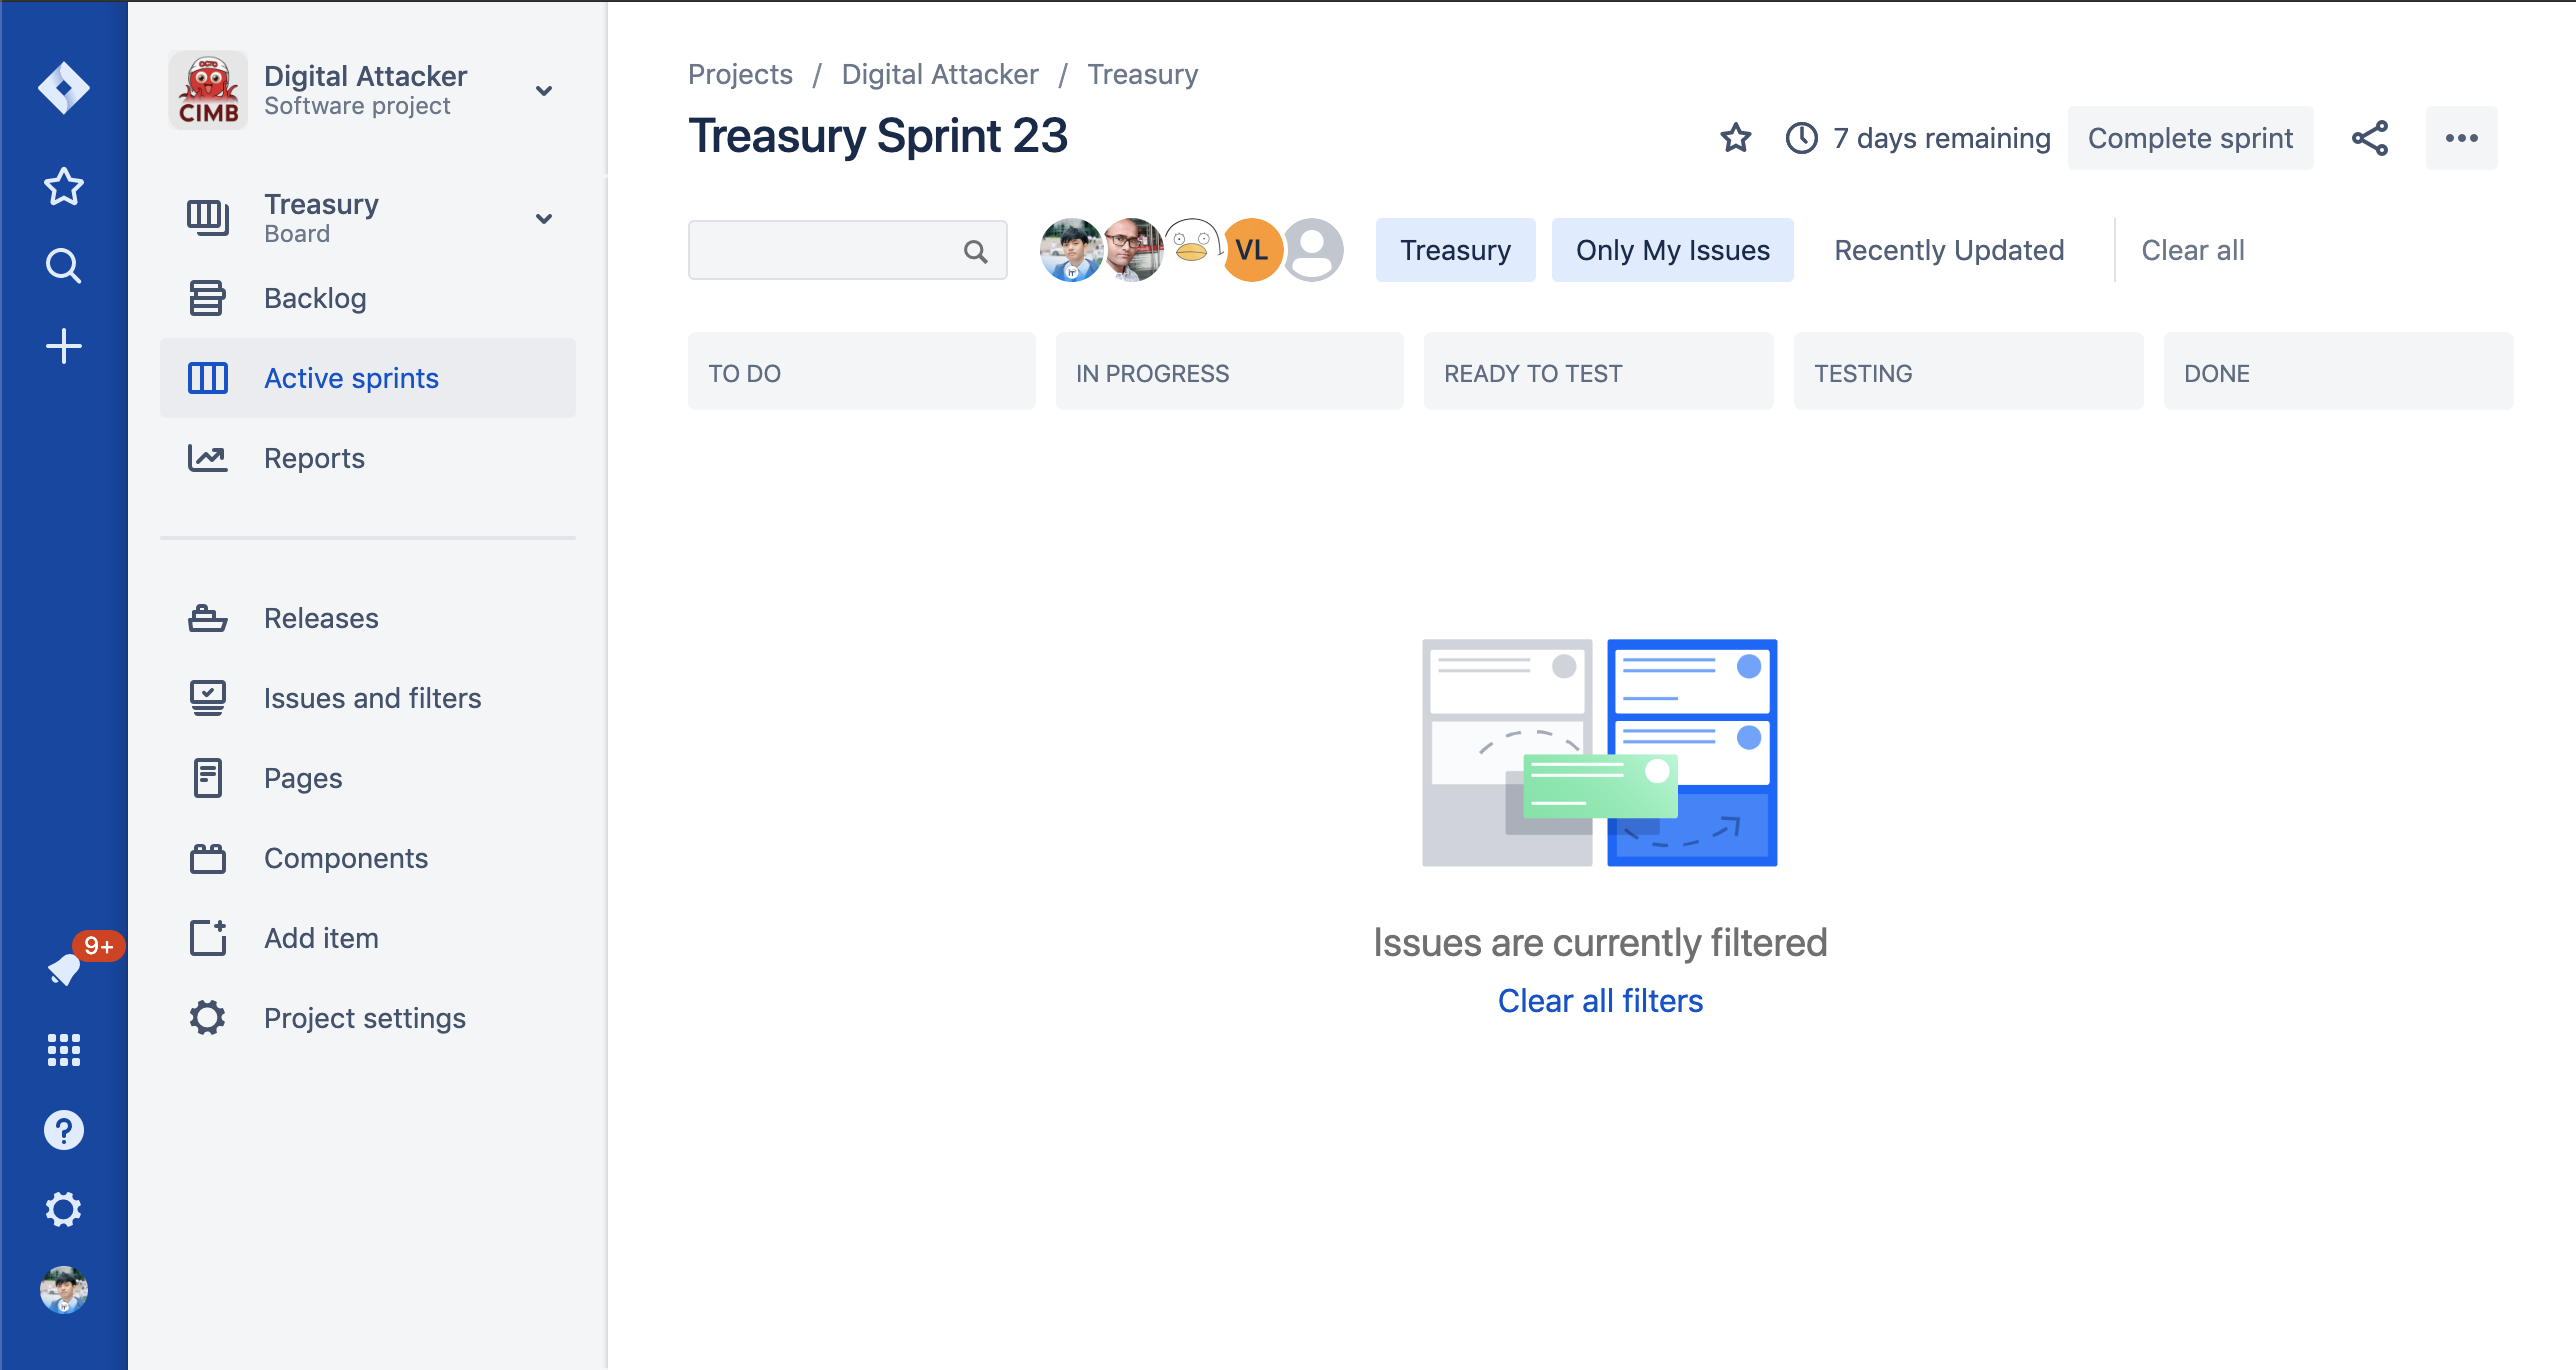
\includegraphics[width=1\textwidth]{jira}
            \caption{หน้าการใช้งาน Jira Software}\label{jira}
        \end{figure}
        โปรแกรมติดตามและแก้ไขปัญหา โดยใช้หลักการของ Agile จัดทำขึ้นเพื่อใช้ในการแก้ไขความผิดพลาดของโปรแกรม (Bug) ติดตามปัญหา (Issue Tracking) และใช้ในการบริหารโครงการ (Project Management) พัฒนาโดยบริษัท Atlassion ข้อดีของโปรแกรมมีดังนี้
        \begin{itemize}
            \item[-] สามารถสร้างชิ้นงานได้ (Task) โดยสามารถกำหนดระยะเวลา (Estimate) หรือระดับความสำคัญ (Story Point) และสามารถมอบหมายงานให้แต่ละคนที่อยู่ในทีมได้
            \item[-] สามารถแบ่งรอบการทำงานได้ (Sprint) ซึ่งในแต่ละรอบจะสามารถวางชิ้นงานได้ใน 5 ส่วนคือ งานที่ต้องทำ (To Do) งานที่กำลังดำเนินอยู่ (In Progress) งานที่พร้อมทดสอบ (Ready to Test) งานที่ที่กำลังทดสอบ (Testing) และงานที่เสร็จแล้ว (Done) โดยระหว่างที่รอบการทำงานยังไม่จบ สามารถที่จะลากชิ้นงานไปมาในได้ตลอด หากมีการแก้ไข
            \item[-] เมื่อจบรอบการทำงานแล้ว จะมีแผนภูมิในแบบต่างๆ (Chart) สรุปผลการทำงานให้ ตามหลักของ Agile แล้ว นิยมใช้ Burndown Chart
        \end{itemize}

    \subsection{Jenkins}
    \begin{figure}[H]
        \centering
        
\includegraphics[width=0.2\textwidth]{jenkins-logo}
        \caption{ตราสัญลักษณ์ Jenkins}\label{jenkins-logo}
    \end{figure}
    Open Source Tools ที่ถูกเขียนด้วยภาษา Java ครับ โดย Jenkins ถูกสร้างขึ้นมาเพื่อตอบสนอง Concept 2 อย่างหลักๆ คือ 
    Continuous integration และ Continuous Delivery โดยการรันเทสของเรานั้นจะเป็นการนำไปผูกอยู่กับ Flow ของ Continuous integration\cite{jenkins}

\section{ลักษณะขั้นตอนการทำงาน}
รูปแบบการทำงานใช้แบบ Agile โดยใช้โครงสร้างการทำงานแบบ Scrum ซึ่งก็คือทำเป็นวงรอบ (Sprint) ซึ่งแต่ละ Sprint จะมีระยะเวลา 3 สัปดาห์ โดยในแต่ละ Sprint จะรายละเอียดการทำงานดังนี้
\subsection{Product Backlog Grooming}
เป็นวันแรกของสัปดาห์ที่หนึ่งที่ทุก ๆ คนในทีมมาดูว่าใน Product Backlog มีงาน(Story)อะไรบ้างแล้วรายละเอียดแต่ละงาน(Story)เป็นยังไงมีส่วนไหนต้องทำบ้างไม่ว่าจะเป็น Frontend หรือ Backend โดยจะมีการ Estimate แต้มกันจนกว่าทุกคนจะให้แต้มเท่ากันโดยแต้มมีลำดับการให้เป็นลำดับ Fibonacci ถ้าให้ไม่เท่ากันก็จะถามเหตุผลในการให้แต้ม แล้ว Re-Estimate กันใหม่จนแต้มเท่ากันทุกคน

    \subsection{Sprint Planning}
    เป็นวันที่สองของสัปดาห์ที่นักพัฒนาจะทำการออกแบบ Sequence Diagram ของ Backend ว่าจะติดต่อกับ Mobile ยังไงแล้ว Flow แต่ละ Flow จะมี Request, Response อะไรบ้าง และมีการ Planning ในส่วนของ UI ที่ซับซ้อนเพื่อที่จะได้รองรับกรณี Error ได้ทั่วถึง 
        
    \subsection{Develop And Test}
    เป็นวันเริ่ม Sprint ที่ นักพัฒนาสามารถเริ่มต้นพัฒนาแอปพลิเคชันได้โดยการพัฒนานั้นนักพัฒนาคนนั้น ๆ ต้องทำการสร้างชุดทดสอบของส่วนที่ตัวเองนั้นพัฒนาด้วยโดยจะเริ่มตั้งวันที่สามของ Sprint ไปจนถึงวันสุดท้ายของสัปดาห์ที่สองโดยผู้ทดสอบแอปพลิเคชันระหว่างพัฒนาอยู่คือ Quality Assurance เพื่อหาจุดผิดพลาด(Bug) แล้วแจ้งนักพัฒนาแก้ไข

    \subsection{Daily Stand-up}
    เป็นกิจกรรมที่จะมีการมาอัพเดทงานและปัญหาที่เจอในวันก่อน ๆ และบอกสิ่งที่จะทำในวันนี้ซึ่งจะทำในทุก ๆ เช้าของวันทำงาน

    \subsection{Product Backlog Refinement}
    เป็นวันแรกของสัปดาห์ที่สองที่หัวหน้านักพัฒนาจะไปคุยว่างาน Sprint นี้สามารถทำทันไหมแล้วต้องการเอางานออกหรือเข้าตามความหมาะสม

    \subsection{Sprint Review}
    เป็นวันที่ 2 ของสัปดาห์ที่สามที่นักพัฒนามาสาธิตในงานที่ทำใน Sprint นี้หลังจากที่พัฒนา และทดสอบแล้วให้กับ Product Owner (PO) และ Project Manager (PM) เพื่อที่จะให้ PO และ PM ไปนำเสนอแอปพลิเคชันที่พัฒนาใน Sprint นี้กับทีม Business เพื่อให้ทีม Business ดูว่าตรงตามความต้องการมากน้อยแค่ไหน
    
    \subsection{Release Code Day}
    เป็นวันที่นักพัฒนาจะทำการอัปโหลดหรือปล่อยแอปพลิเคชันที่ทำใน Sprint นี่ขึ้นสู่สภาพแวดล้อม และ Server ของ User Acceptance Testing
    
    \subsection{User Acceptance Testing}
    User Acceptance Testing: เป็นวันที่ Quality Assurance หรือ QA จะทำการทดสอบแอปพลิเคชันโดยการจำลองเป็นลูกค้าแล้วหาจุดผิดพลาดเพื่อให้นักพัฒนาแก้ไขโดยจะเริ่มตั้งแต่วันที่ 3 ของสัปดาห์ที่สามจนถึงวันสุดท้ายของสัปดาห์ที่สาม

    \subsection{PI Planning}
    เป็นวันใดวันหนึ่งก็ได้ใน Sprint ที่หัวหน้านักพัฒนาจะคุยกับ Product Owner ถึง Product Backlog ใน Sprint ว่าจะต้องทำอะไรบ้างความต่้องการทางธุรกิจที่ไปเจรจาและรวบรวมมาจากทีม Business
            
    \subsection{Sprint Retrospective}
    เป็นวันสุดท้ายของสัปดาห์ที่สามที่ทุก ๆ คนในทีมไม่ว่าจะเป็น นักพัฒนา, หัวหน้านักพัฒนา, Quality Assurance, Project Manager และ Product Owner จะมาพูดถึงเรื่องราวต่าง ๆ ที่เกิดขึ้นใน Sprint ที่ผ่านมาไม่ว่าจะเป็นเรื่องงาน หรือเรื่องความเป็นอยู่ของคนในทีมโดยทาง Digital Banking จะเลือกใช้รูปแบบการ Retrospective เป็น Good, Bad, Try และ Next Action เพื่อที่จะมาบอกว่ามีอะไรบ้างที่ถือเป็นเรื่องดีไม่ดีใน Sprint นี้และมีอะไรที่ต้องพยายามให้มากขึ้นใน Sprint ถัดไปแล้ว Facilitator จะเป็นคนให้คนในทีมโหวตเพื่อเลือก Next Action มาสองอย่างจากเรื่องที่มีคนโหวตมากที่สุด

